Solar radiation on Mars is made of beam and diffuse components. Designing \ac{PV} power systems for surface operations requires an understanding of the characteristics of these components as well as how they are affected by the Martian atmosphere.

\subsection{Seasons}
\label{sec:MartianEnvironment:Seasons}
The red planet's axis is tilted away from the sun at \SI{25}{\degree}. Very much like Earth's \SI{23.5}{\degree} axial tilt, this results in seasons. Mars has an orbit with a semi-major axis of 1.524 \si{\astronomicalunit} which translates to a Martian year corresponding to an orbital period of 687 days. Its eccentricity is 0.0934 which contributes to aphelion and periphelion distances of 1.666 \si{\astronomicalunit} and 1.3814 \si{\astronomicalunit}, respectively. Martian seasons are longer and 1.88 Earth years go by for every Martian year. Sidereal days are 24.62 hours long and solar days are 24.65 hours long.

\begin{table}[H]
  \footnotesize
  \centering
  \caption{Seasonal advances on Mars.}
  \label{tab:mars-seasonal-advances}
  \begin{tabular}{|l|l|l|}
  \hline
  \multirow{2}{*}{\textbf{\begin{tabular}[c]{@{}l@{}}Areocentric\\ Longitude\end{tabular}}} & \multicolumn{2}{c|}{\textbf{Seasonal Advance}} \\ \cline{2-3}
   & \multicolumn{1}{c|}{\textbf{Northern Hemisphere}} & \multicolumn{1}{c|}{\textbf{Southern Hemisphere}} \\ \hline
  \si{0}{\degree} & Vernal Equinox & Autumnal Equinox \\ \hline
  \si{0}{\degree} to \si{90}{\degree} & Spring & Autumn \\ \hline
  \si{90}{\degree} & Summer Solstice & Winter Solstice \\ \hline
  \si{90}{\degree} to \si{180}{\degree} & Summer & Winter \\ \hline
  \si{180}{\degree} & Autumnal Equinox & Vernal Equinox \\ \hline
  \si{180}{\degree} to \si{270}{\degree} & Autumn & Spring \\ \hline
  \si{270}{\degree} & Winter Solstice & Summer Solstice \\ \hline
  \si{270}{\degree} to \si{360}{\degree} & Winter & Summer \\ \hline
  \end{tabular}
\end{table}


A Martian day, known as a Sol, is approximately 40 minutes longer than an Earth day. Mars' position on its orbit is described in terms of areocentric longitude of the Sun, $L_{s}$, and is measured Eastwards from $L_{s} = \SI{0}{\degree}$ at the northern hemisphere's Vernal equinox. The transition of Martian seasons are presented in \refTab{tab:mars-seasonal-advances} with respect to areocentric longitudes.

\subsection{Dust}
\label{sec:MartianEnvironment:Dust}
The Martian surface is aeolianly active with varying concentration of airborn dust throughout the year due to processes of dust lifting, transportation, and deposition \citemarsenv{Kahre2006}.

\begin{figure}[h]
\captionsetup[subfigure]{justification=centering}
%\vspace{-2ex}
\centering
    %% kill hyper-link highlighting
    \hypersetup{hidelinks=true}%
    %% the figures
    \begin{subfigure}[t]{0.55\textwidth}
        \centering
            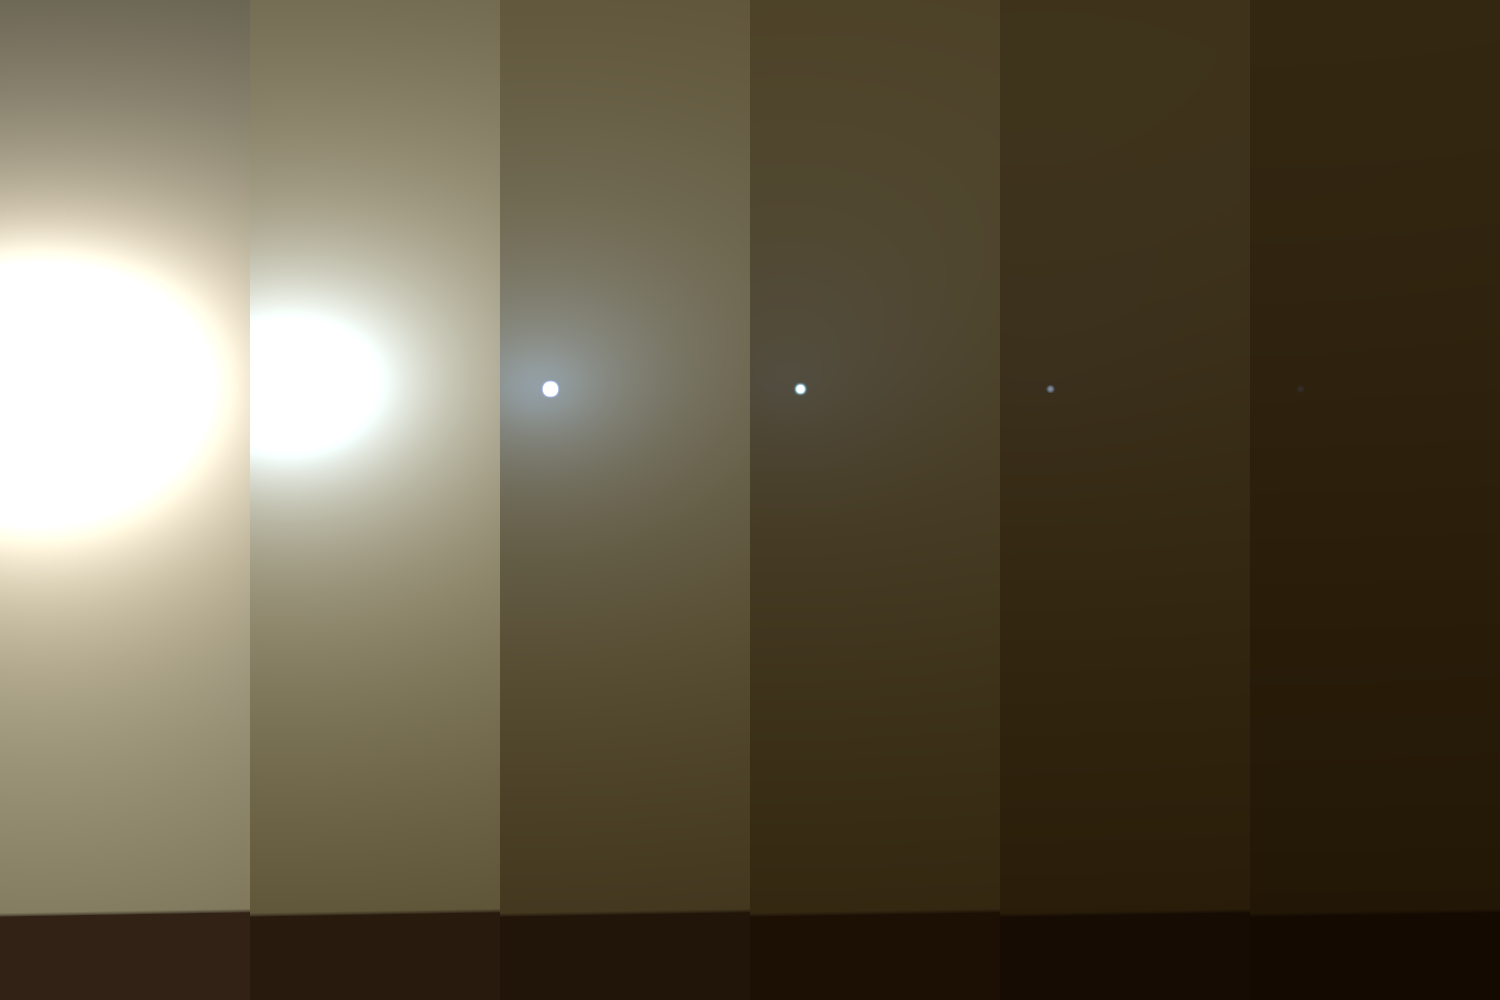
\includegraphics[height=50mm]{sections/mars-solar-energy/solar-radiation/images/tau-factors.png}
            \subcaption{Simulated views of atmospheric dust opacity}
            \label{fig:image:tau-factors}
    \end{subfigure}\hfill%
    \begin{subfigure}[t]{0.45\textwidth}
        \centering
            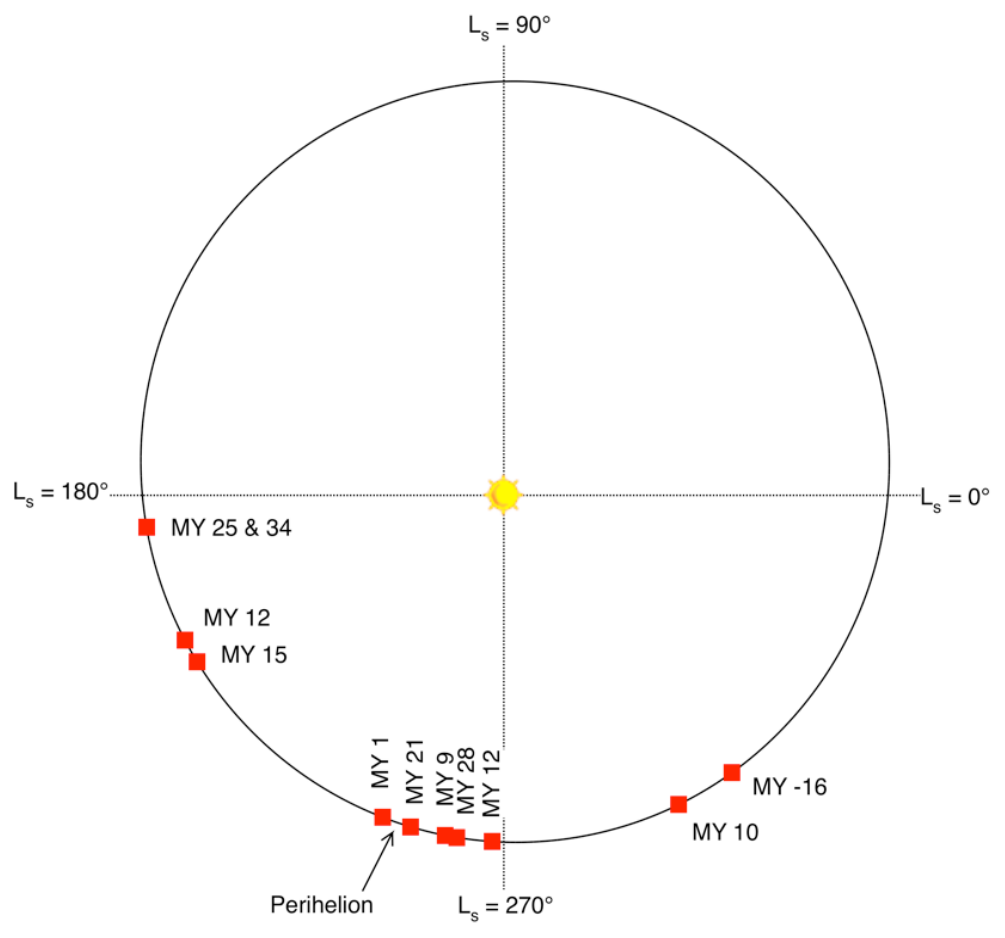
\includegraphics[height=50mm]{sections/mars-solar-energy/solar-radiation/images/timin-of-observed-global-dust-storms.png}
            \subcaption{Global dust storm timing}
            \label{fig:image:global-dust-storm-timing}
    \end{subfigure}
    \caption[Simulated views of dusty atmosphere and timing of global dust storms]
    {Simulated views of dusty atmosphere and timing of global dust storms. (a) From left to right, $\tau$ factors of 1, 3, 5, 7, 9, and 11. Image: NASA/JPL-Caltech/TAMU. (b) Timing of observed global dust storms is concentrated in the season near the periphelion. Taken from \citemarsenv{Smith2019}.}
    \label{fig:dust}
\vspace{-2ex}
\end{figure}

\subsubsection{Atmospheric Opacity}
\label{sec:MartianEnvironment:Dust:AtmosphericOpacity}
The density of suspended dust determines the atmospheric opacity, or optical depth, measured in $\tau$ factors. A $\tau$ factor between 0 and 0.5 indicates a clear to relatively clear day. Higher $\tau$ factors indicate dusty days with growing atmospheric dust opacity as represented in \refFig{fig:image:tau-factors} for simulated views pointing towards the Sun. %\SI{99}{\percent} of sunlight is blocked at $\tau$ factor 4.7.

\subsubsection{Storms}
\label{sec:MartianEnvironment:Dust:Storms}

Dust storms are likely to occur while Mars approaches the Sun during the periphelion season between $L_{s} = \SI{185}{\degree}$ and $L_{s} = \SI{315}{\degree}$ \citemarsenv{Smith2019}. The Sun's proximity warms the atmosphere which creates temperature differences that produce dust lifting winds. The process is exacerbated by the release of carbon dioxide from the evaporating winter polar cap which thickens the atmosphere and increases surface pressure so that dust particles remain airborn. \refFig{fig:image:global-dust-storm-timing} shows the the timing of global dust storms until \ac{MY} 34.

Global dust storms that cover an area of over \SI{e7}{\kilo\meter\squared} have a yearly probability of \SI{30}{\percent} to \SI{80}{\percent} whereas local dust storms that cover an area less than \SI{e7}{\kilo\meter\squared} occur with a \SI{5}{\percent} probability \citepower{Kerslake1999}. Local dust storms typically have $\tau \approx 1$ \citepower{Kerslake1999} whereas the largest in situ $\tau$ factor recorded by \ac{MER} Opportunity was 10.8 in \ac{MY}34 near $L_{s} = \SI{180}{\degree}$.

\subsection{Solar Radiation}
\label{sec:MartianEnvironment:SolarRadiation}

The Martian surface radiation profiles showcased throughout this section are for a planetary latitudes of \SI{2}{\degree}S, \SI{34}{\degree}S, and \SI{34}{\degree}N. Equations presented in this section as well as their nomenclatures are taken from \citemarsenv{Appelbaum1989}, \citemarsenv{Appelbaum1990}, \citemarsenv{Appelbaum1991}, \citemarsenv{Appelbaum1993}, and \citemarsenv{Appelbaum1994} where profiles at \ac{VL1} and \ac{VL2} locations are presented.

\subsubsection{Irradiance}
\label{sec:MartianEnvironment:SolarRadiation:Irradiance}

Beam irradiance is the total solar flux density expressed in \si{Wm^{-2}}. It is a measure of solar radiation from direct sunlight. At the top of the Martian atmosphere the instantaneous beam irradiance, $G_{ob}$, is a function the areocentric longitude $L_{s}$ and is shown in \refEqn{eq:G_ob}.

\begin{equation}
  \label{eq:G_ob}
  G_{ob} = 590 \frac{[1 + e \cos{(L_{s} - 248)}]^2}{(1-e^2)^2}
\end{equation}

Where \SI{590}{Wm^{-2}} is the mean beam irradiance at the top of the Martian atmosphere, $L_{s} - \SI{248}{\degree}$ is the true anomaly, and $e$ is the Mars eccentricity. The variation of $G_{ob}$ is presented in \refFig{fig:plot:beam-irradiance-top-of-mars-atmosphere}. At its closest, during the perihelion at $L_{s} = \SI{248}{\degree}$, Mars is at a distance of \SI{1.381}{\astronomicalunit} from the Sun with an irradiance on top of its atmosphere reaching a maximum of \SI{718}{Wm^{-2}}. At its furthest of 1.67\si{\astronomicalunit}, during the aphelion at $L_{s} = \SI{71}{\degree}$, the irradiance reaches its minimum of \SI{494}{Wm^{-2}}.

\vspace{0.3cm}

\begin{figure}[h]
\captionsetup[subfigure]{justification=centering}
\vspace{-2ex}
\centering
    %% setup sizes
    \setlength{\subfigureWidth}{0.50\textwidth}
    \setlength{\graphicsHeight}{80mm}
    %% kill hyper-link highlighting
    \hypersetup{hidelinks=true}%
    %% the figures
    \begin{subfigure}[t]{\subfigureWidth}
        \centering
            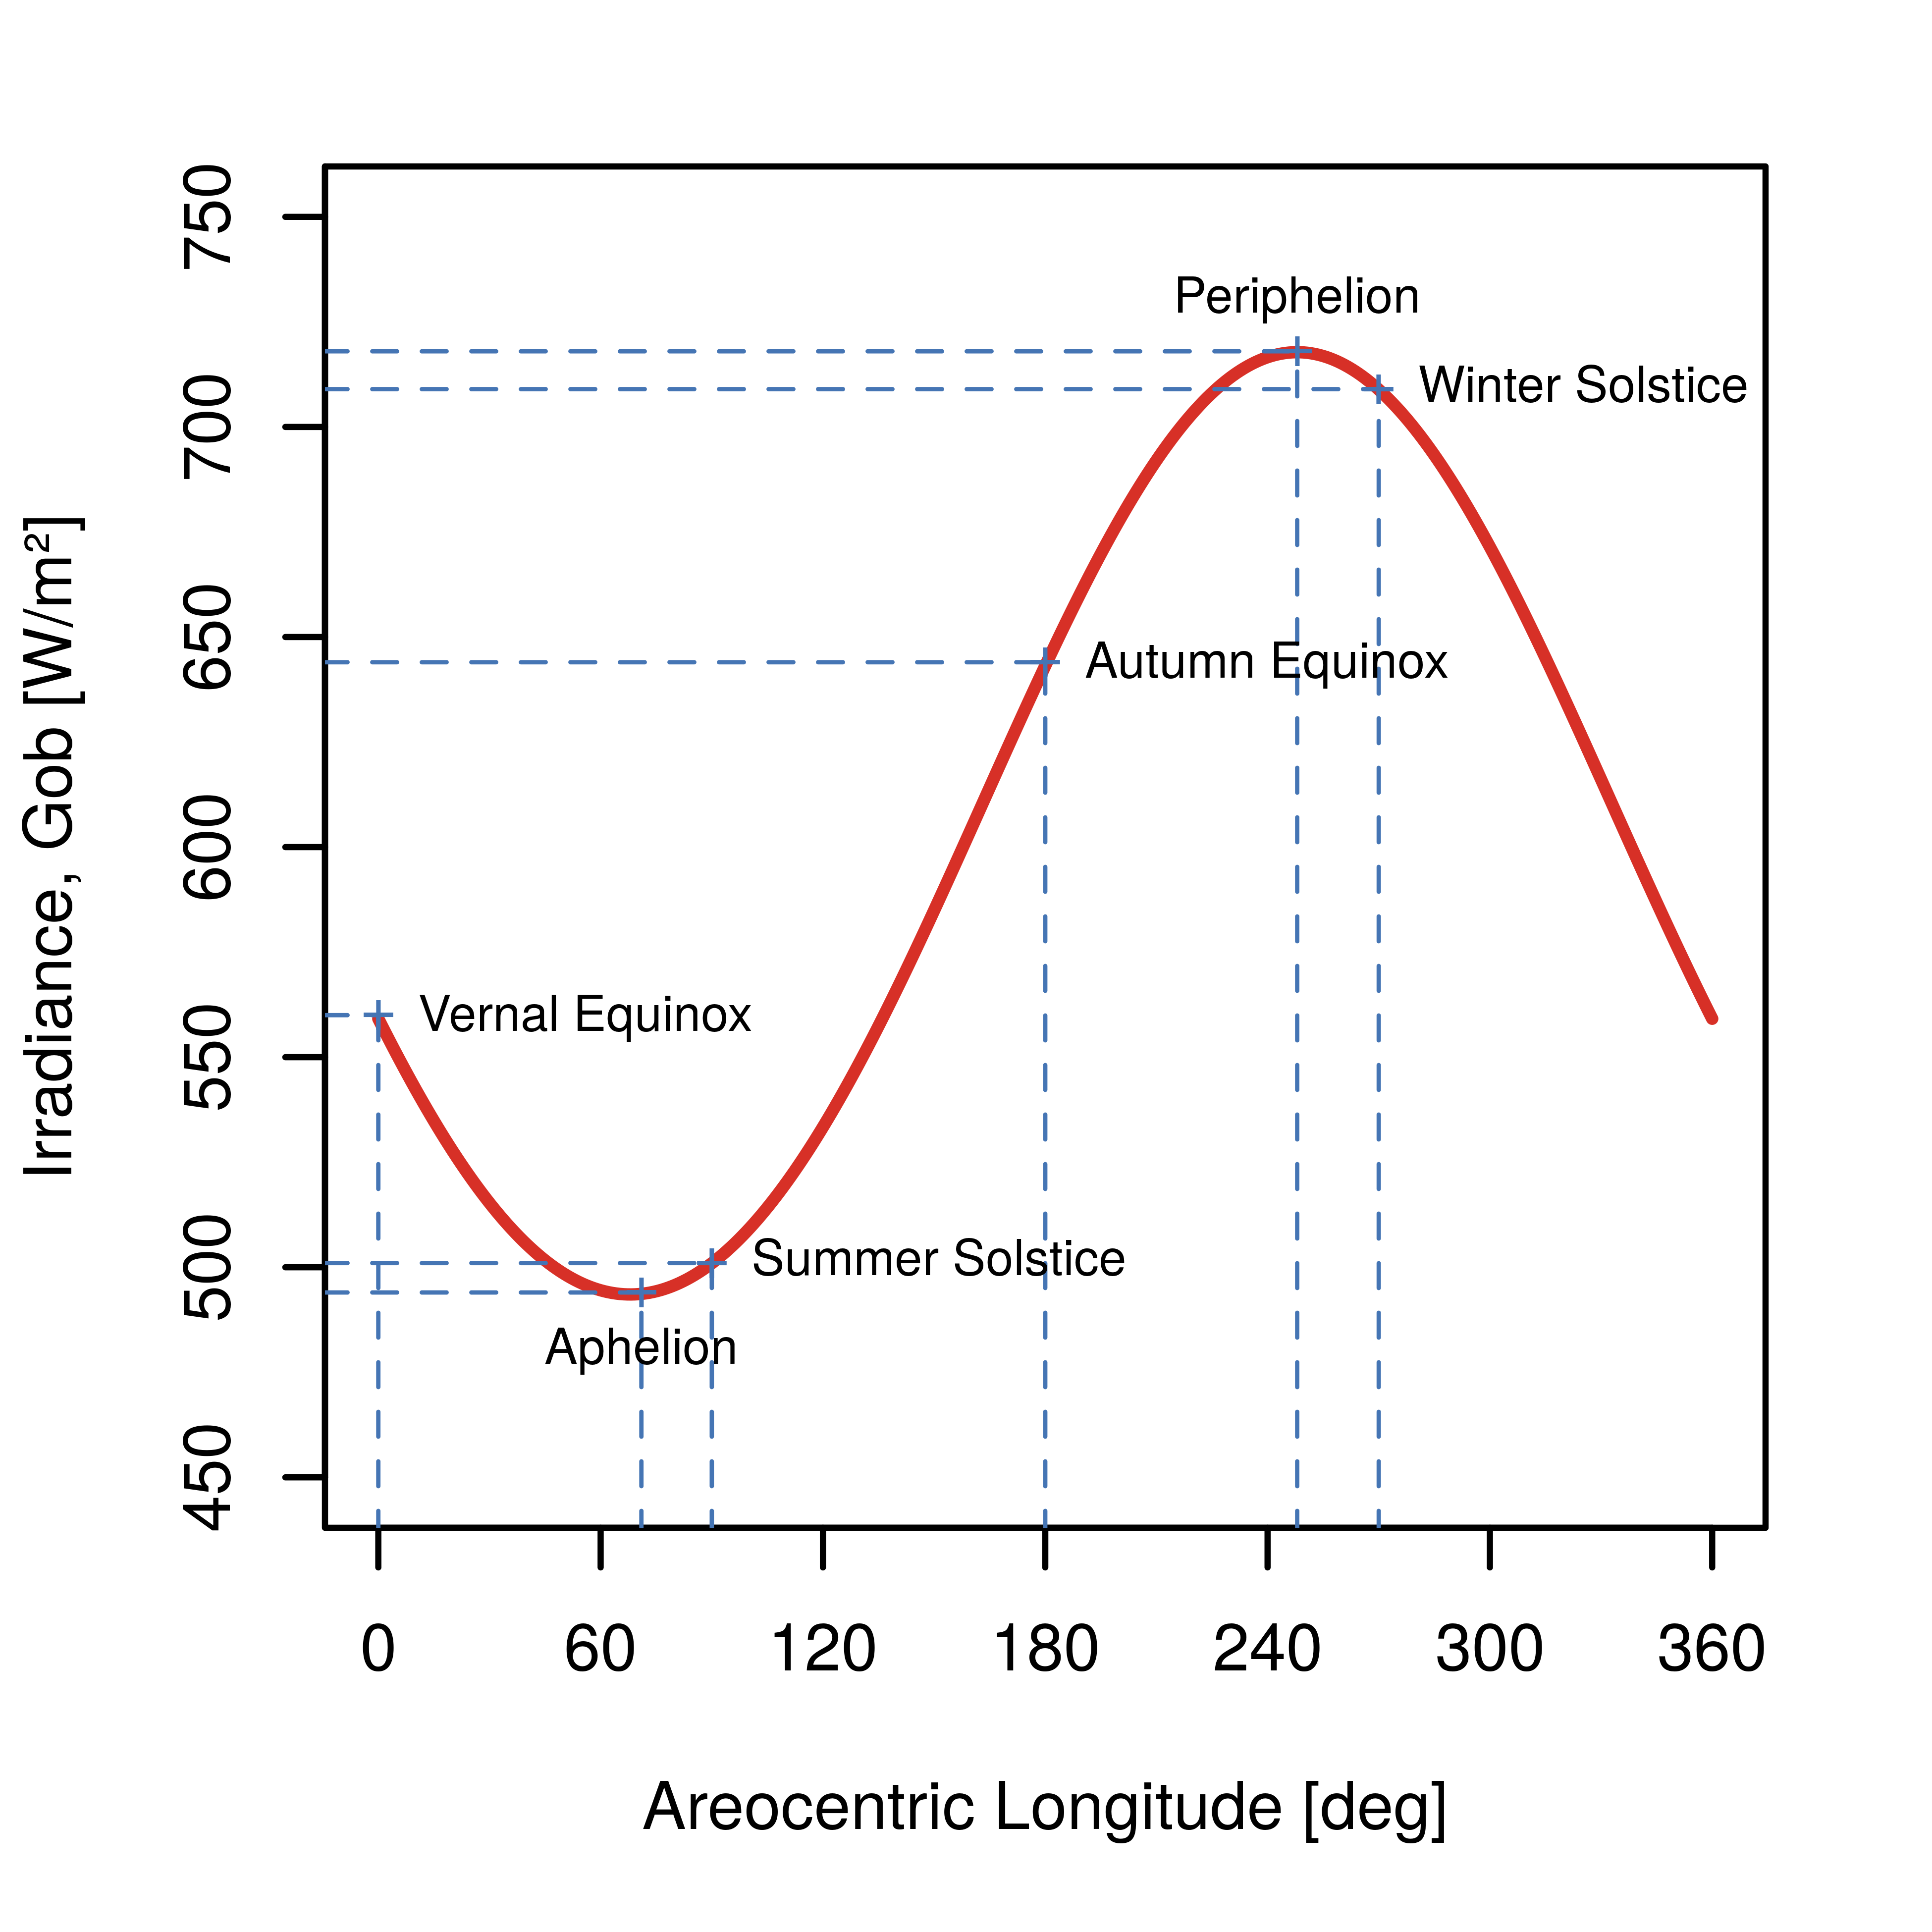
\includegraphics[height=\graphicsHeight]{sections/mars-solar-energy/solar-radiation/plots/gob-daily-variations.png}
            \subcaption{Top of Mars atmosphere}
            \label{fig:plot:beam-irradiance-top-of-mars-atmosphere}
    \end{subfigure}\hfill
    \begin{subfigure}[t]{\subfigureWidth}
        \centering
            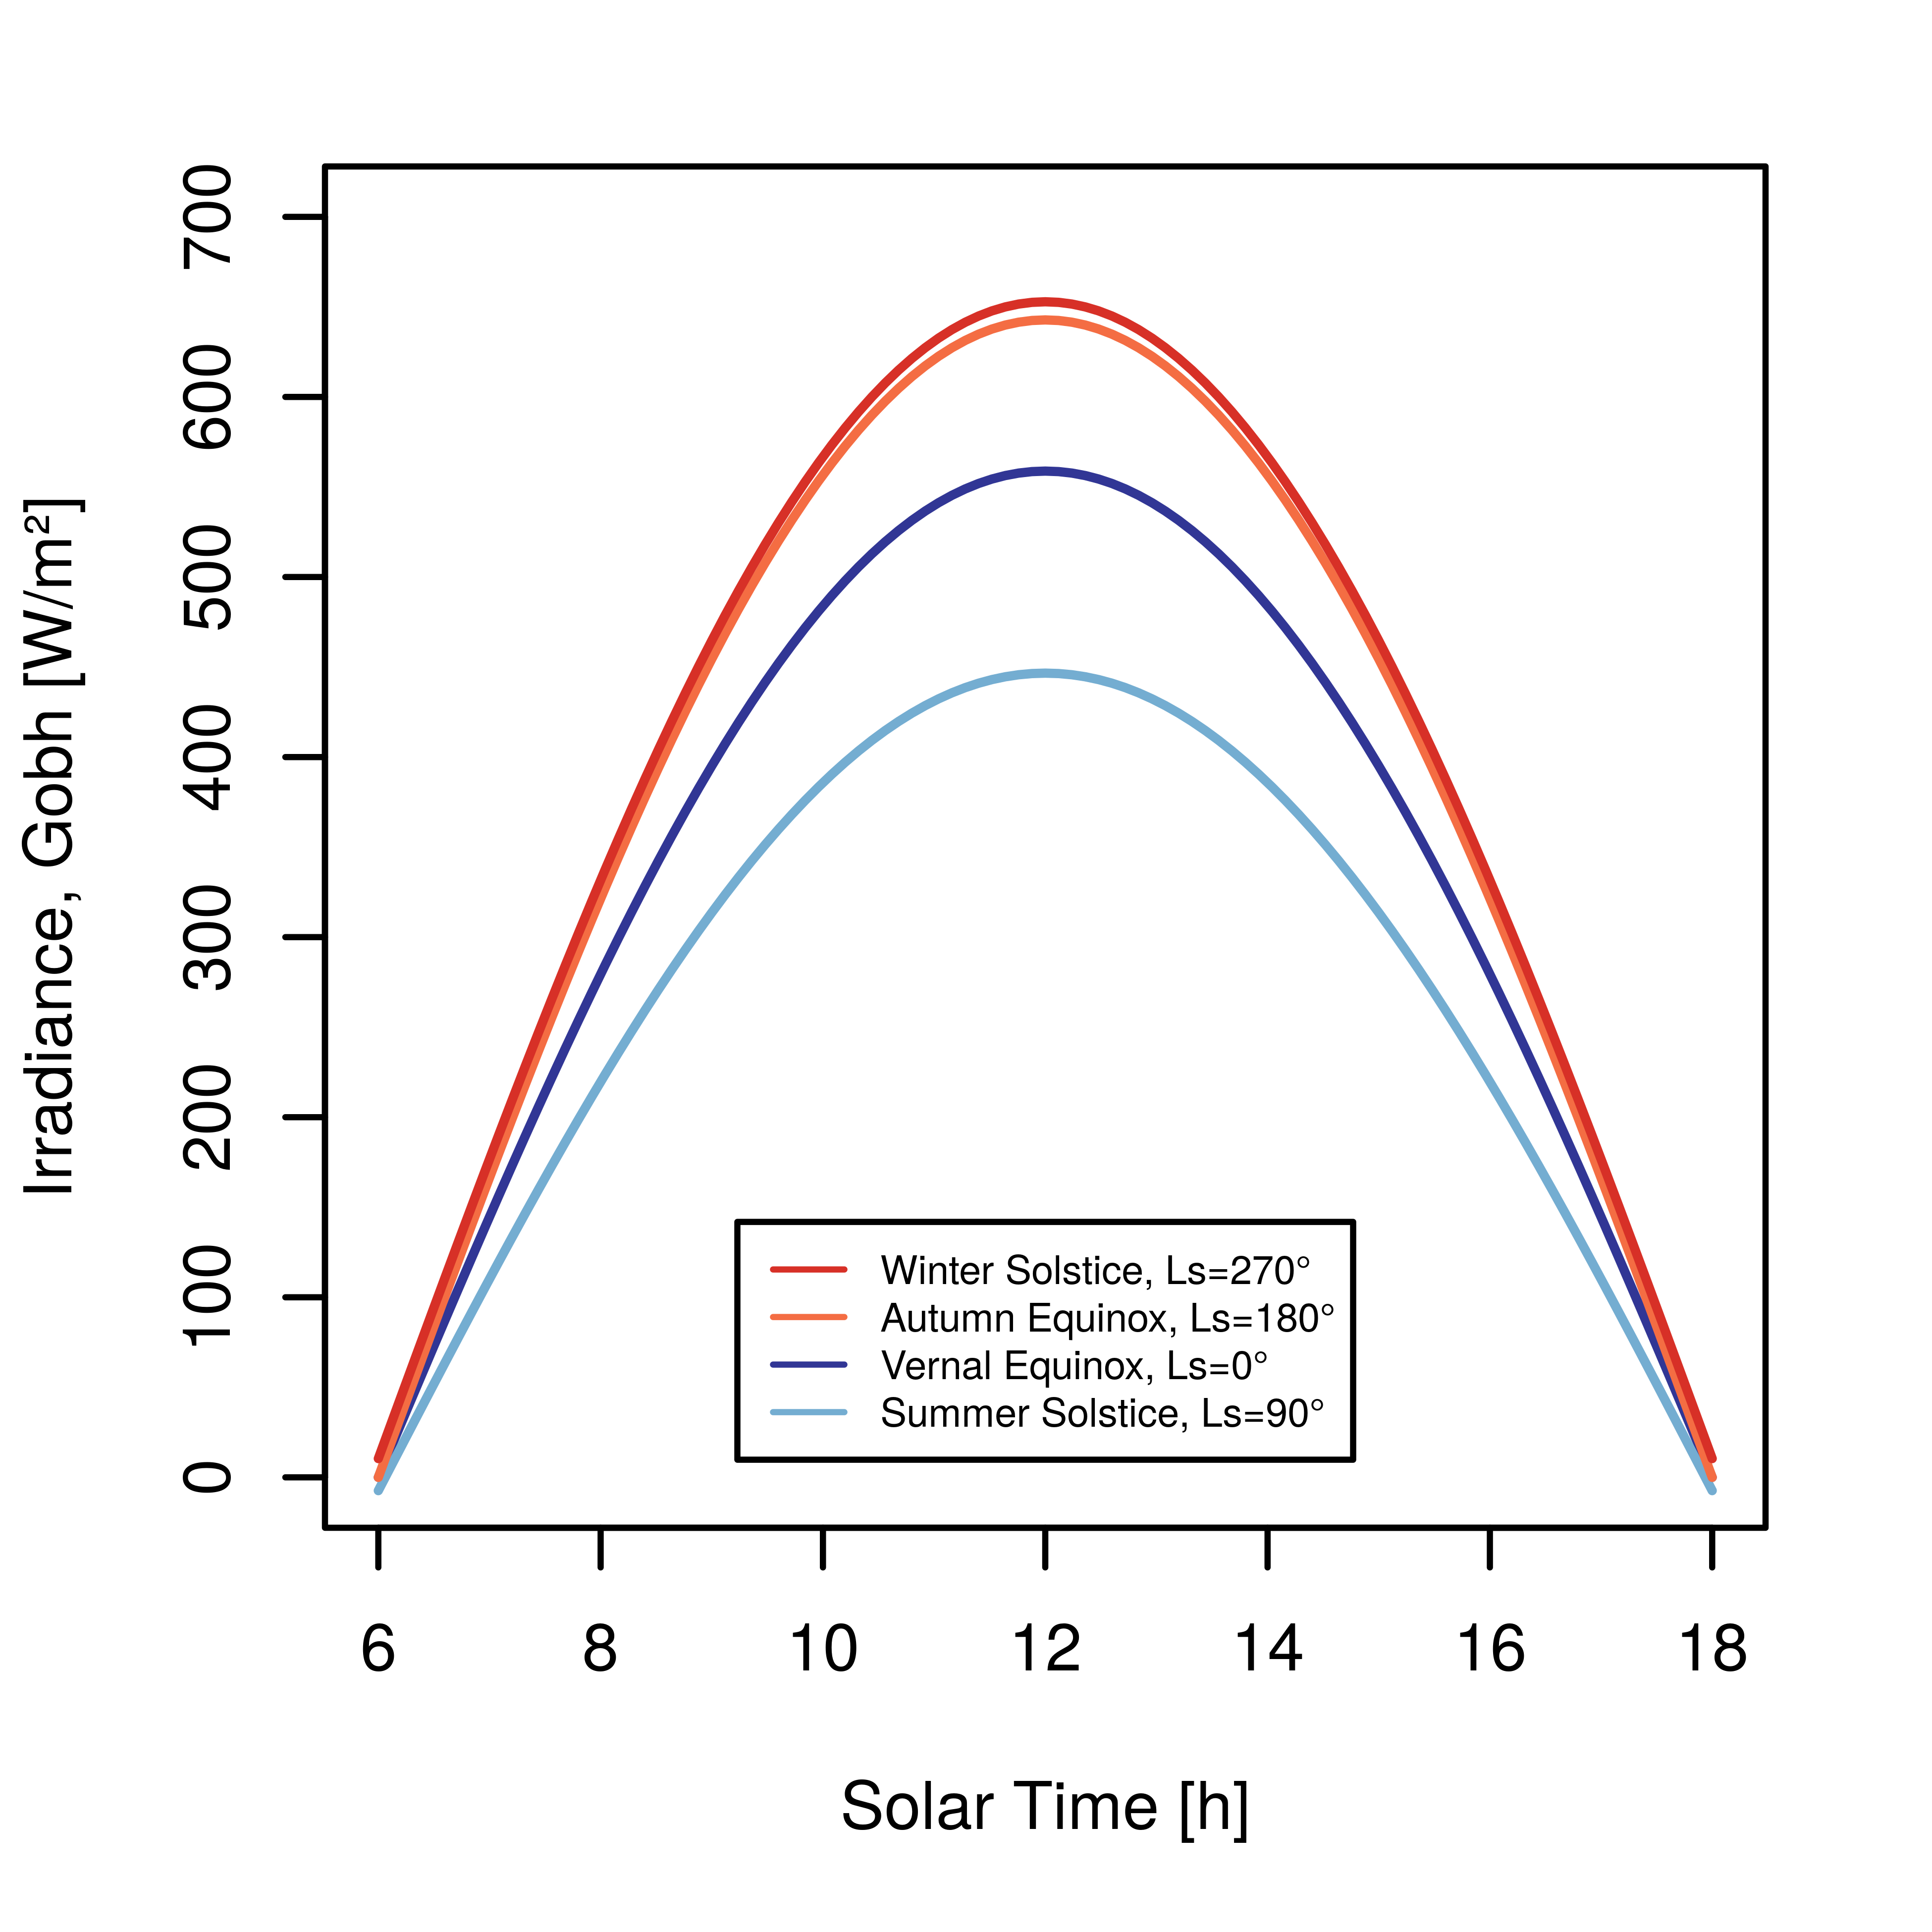
\includegraphics[height=\graphicsHeight]{sections/mars-solar-energy/solar-radiation/plots/gobh-diurnal-over-endaveaour-crater.png}
            \subcaption{Horizontal surface at $\phi=\SI{-2}{\degree}$}
            \label{fig:plot:diurnal-variation-of-beam-irradiance-on-a-horizontal-surface-at-top-of-mars-atmosphere}
    \end{subfigure}\\[0.8ex]
    \caption[Global irradiance variations]
    {Global irradiance variations.}
    \label{fig:plot:global-irradiance}
\vspace{-2ex}
\end{figure}

\vspace{0.3cm}

Further parameterization is necessary in order to measure irradiance on a horizontal surface at the top Mars atmosphere where the solar zenith angle $z$ is considered. The solar zenith angle itself is a function of planetary latitude $\phi$, declination angle $\delta$, and hour angle $\omega$ measured from the true noon westward \citemarsenv{Appelbaum1990}. Expressed as $G_{obh}$, it is presented in \refEqn{eq:G_obh}.

\begin{equation}
  \label{eq:G_obh}
  G_{obh} = G_{ob}\cos{(z)}
\end{equation}

where the Sun zenith angle $z$ is given by \refEqn{eq:cosz}.

\begin{equation}
  \label{eq:cosz}
  \cos{(z)} = \sin{(\phi)}\sin{(\delta)} + \cos{(\phi)}\cos{(\delta)}\cos{(\omega)}
\end{equation}

Solar radiation calculations using \refEqn{eq:G_obh} as a function of solar time are presented in \refFig{fig:plot:diurnal-variation-of-beam-irradiance-on-a-horizontal-surface-at-top-of-mars-atmosphere}. Obtaining the irradiance on the surface of Mars requires the atmospheric opacity $\tau$ as an additional parameter. As shown in \refEqn{eq:G_h_1}, the global irradiance $G_{h}$ is the sum of beam, $G_{bh}$, and diffuse irradiances, $G_{dh}$.

\begin{equation}
  \label{eq:G_h_1}
  G_{h} = G_{bh} + G_{dh}
\end{equation}

The expression for $G_{h}$ and $G_{bh}$ are presented in \refEqn{eq:G_h_2} and \refEqn{eq:G_bh}:

\begin{equation}
  \label{eq:G_h_2}
  G_{h} = G_{ob}\cos{(z)}\frac{f(z,\tau)}{0.9}
\end{equation}

where $f(z,\tau)$ is the normalized net flux function derived from the net solar flux integrated over the solar spectrum on the Martian surface and 0.9 comes from the $(1-albedo)$ expression for an albedo of 0.1 \citemarsenv{Appelbaum1989}.

\begin{equation}
  \label{eq:G_bh}
  G_{bh} = G_{ob}\cos{(z)}\exp\left(\frac{-\tau}{cos{(z)}}\right)
\end{equation}

Diurnal irradiance profiles are presented in \refFig{fig:plot:irradiances-phi} for a clear day during the perihelion. At $L_{s} = \SI{248}{\degree}$, the northern hemisphere is in mid-Autumn whereas the southern hemisphere in mid-Spring. As such, irradiances are much larger at \SI{34}{\degree}S than at \SI{34}{\degree}N.

\begin{figure}[h]
\captionsetup[subfigure]{justification=centering}
%\vspace{-2ex}
\centering
    %% setup sizes
    \setlength{\subfigureWidth}{0.50\textwidth}
    \setlength{\graphicsHeight}{80mm}
    %% kill hyper-link highlighting
    \hypersetup{hidelinks=true}%
    %% the figures
    \begin{subfigure}[t]{\subfigureWidth}
        \centering
            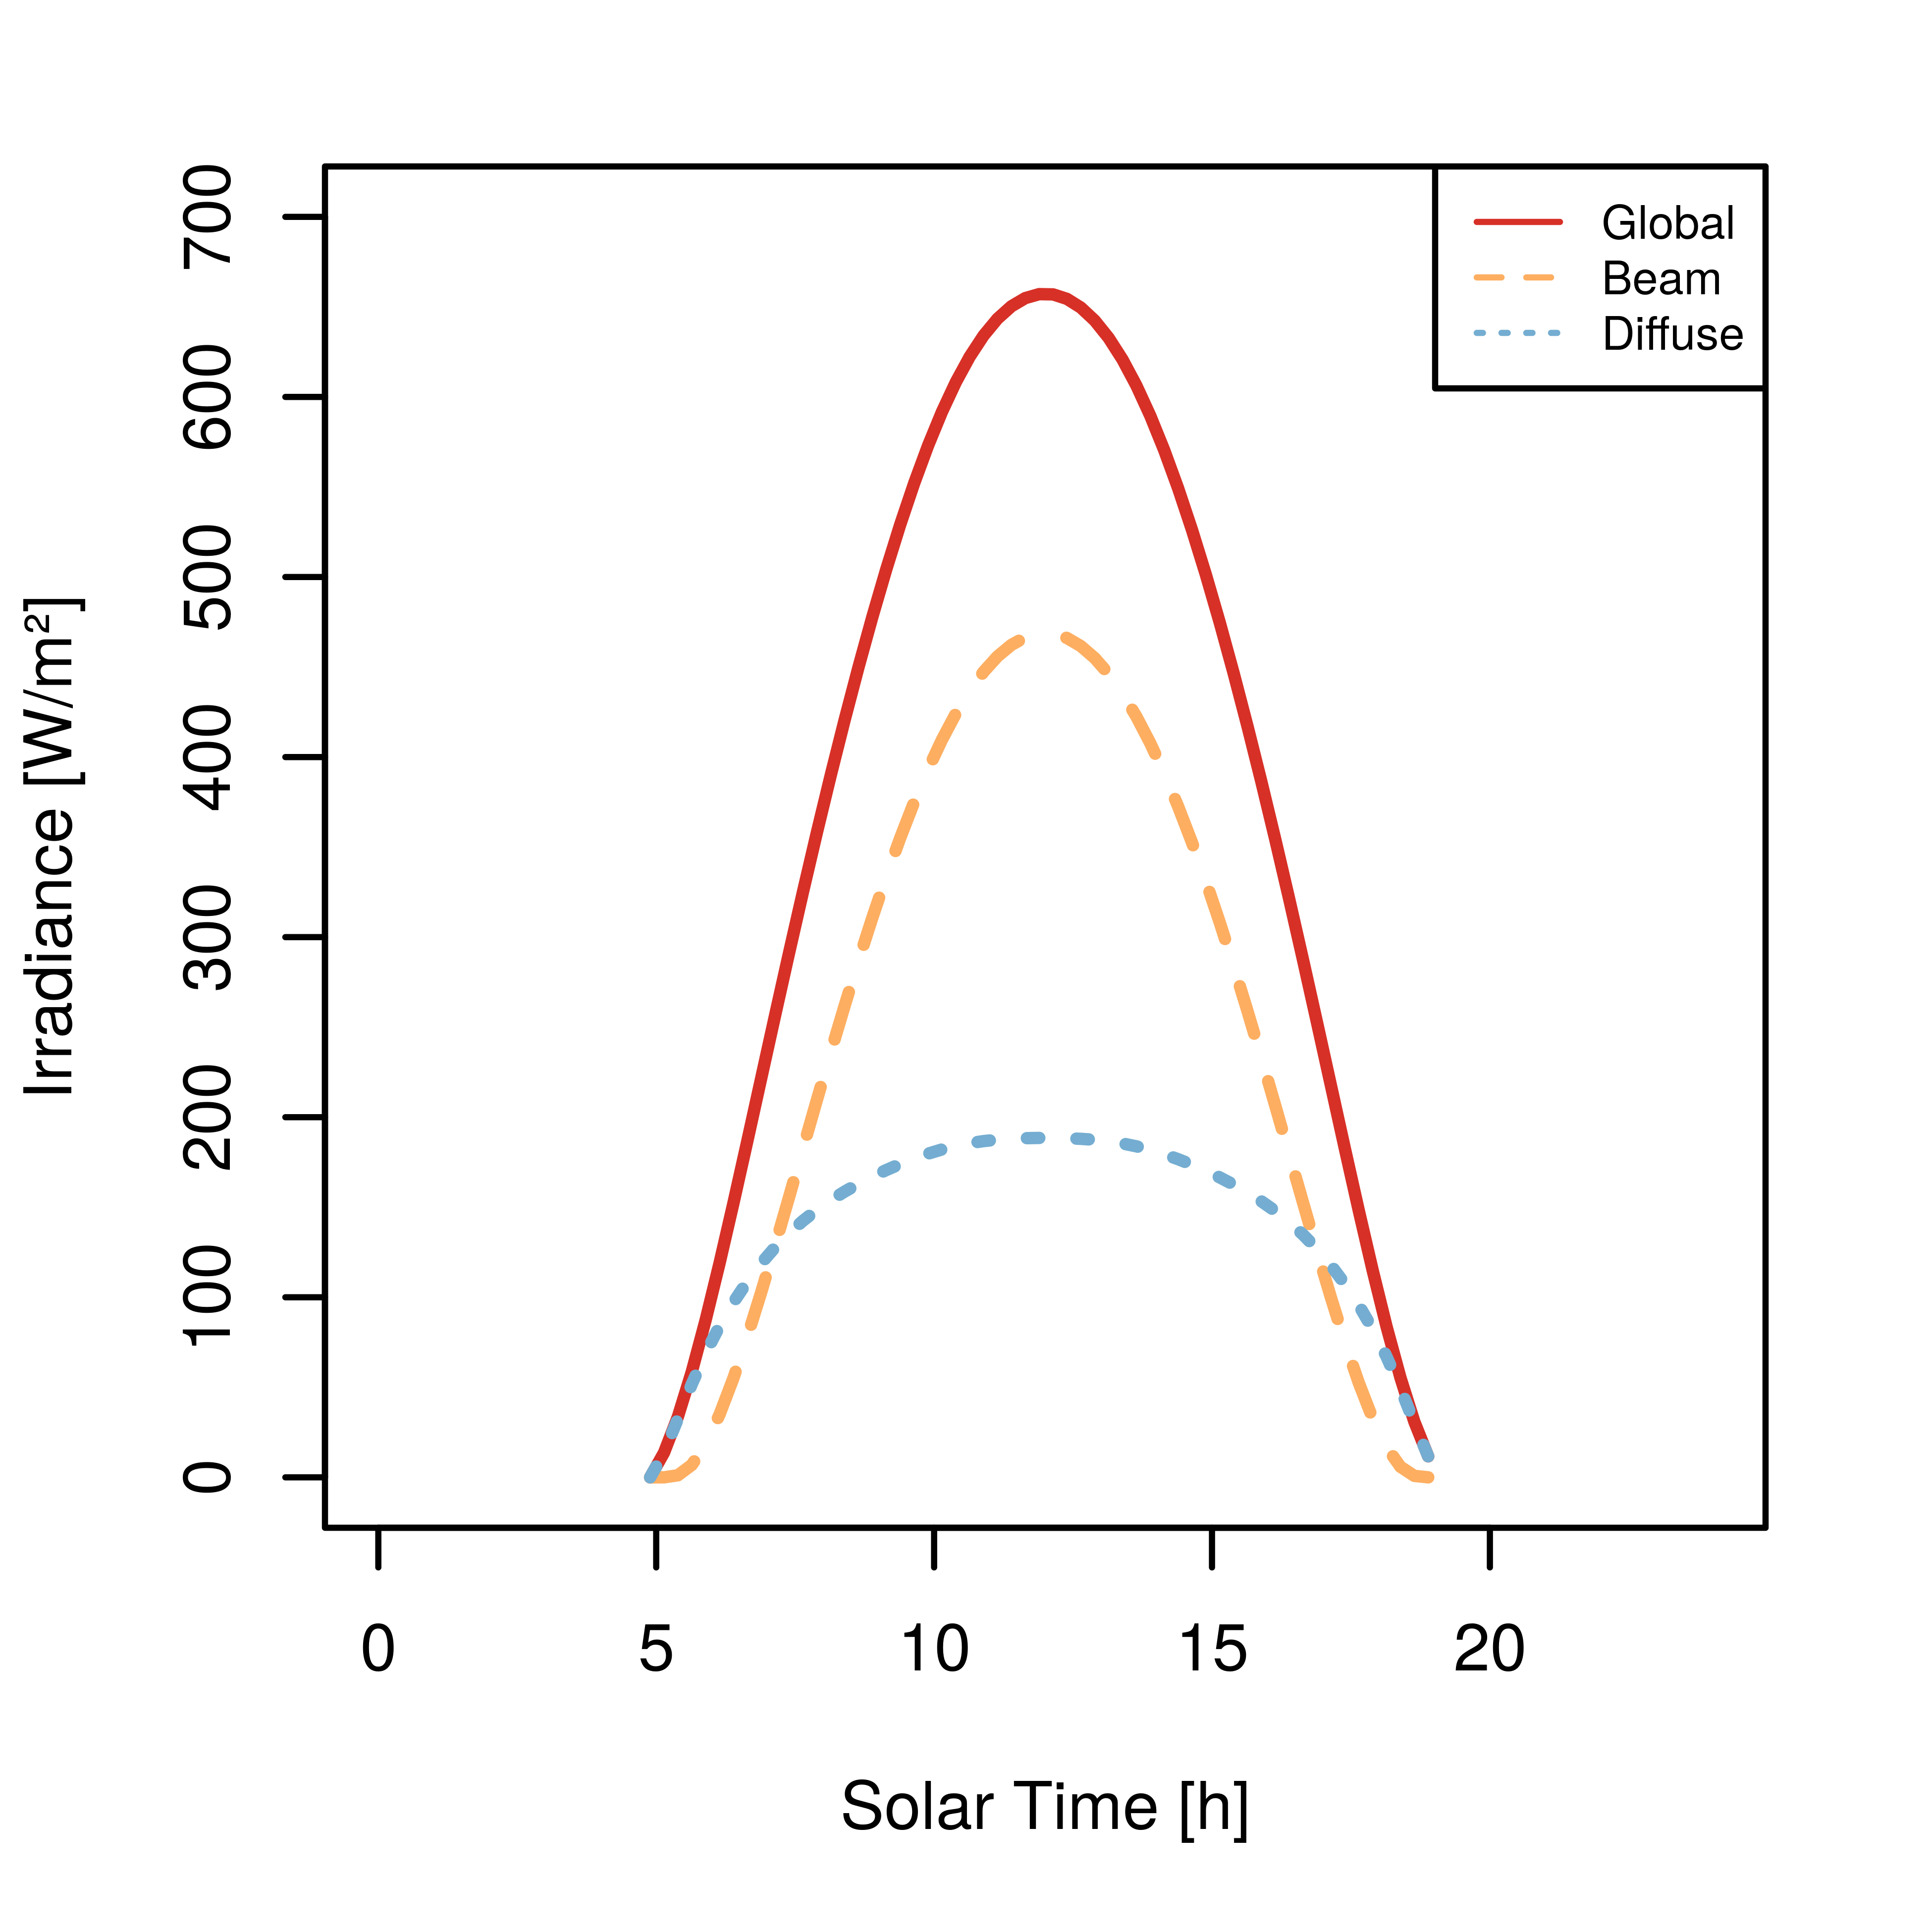
\includegraphics[height=\graphicsHeight]{sections/mars-solar-energy/solar-radiation/plots/gh-gbh-gdh-variation-1-for-ls-248-phi-34-tau-04-and-albedo-027.png}
            \subcaption{$\phi = \SI{-34}{\degree}$}
            \label{fig:plot:sub:irradiance-phi-m34}
    \end{subfigure}\hfill
    \begin{subfigure}[t]{\subfigureWidth}
        \centering
            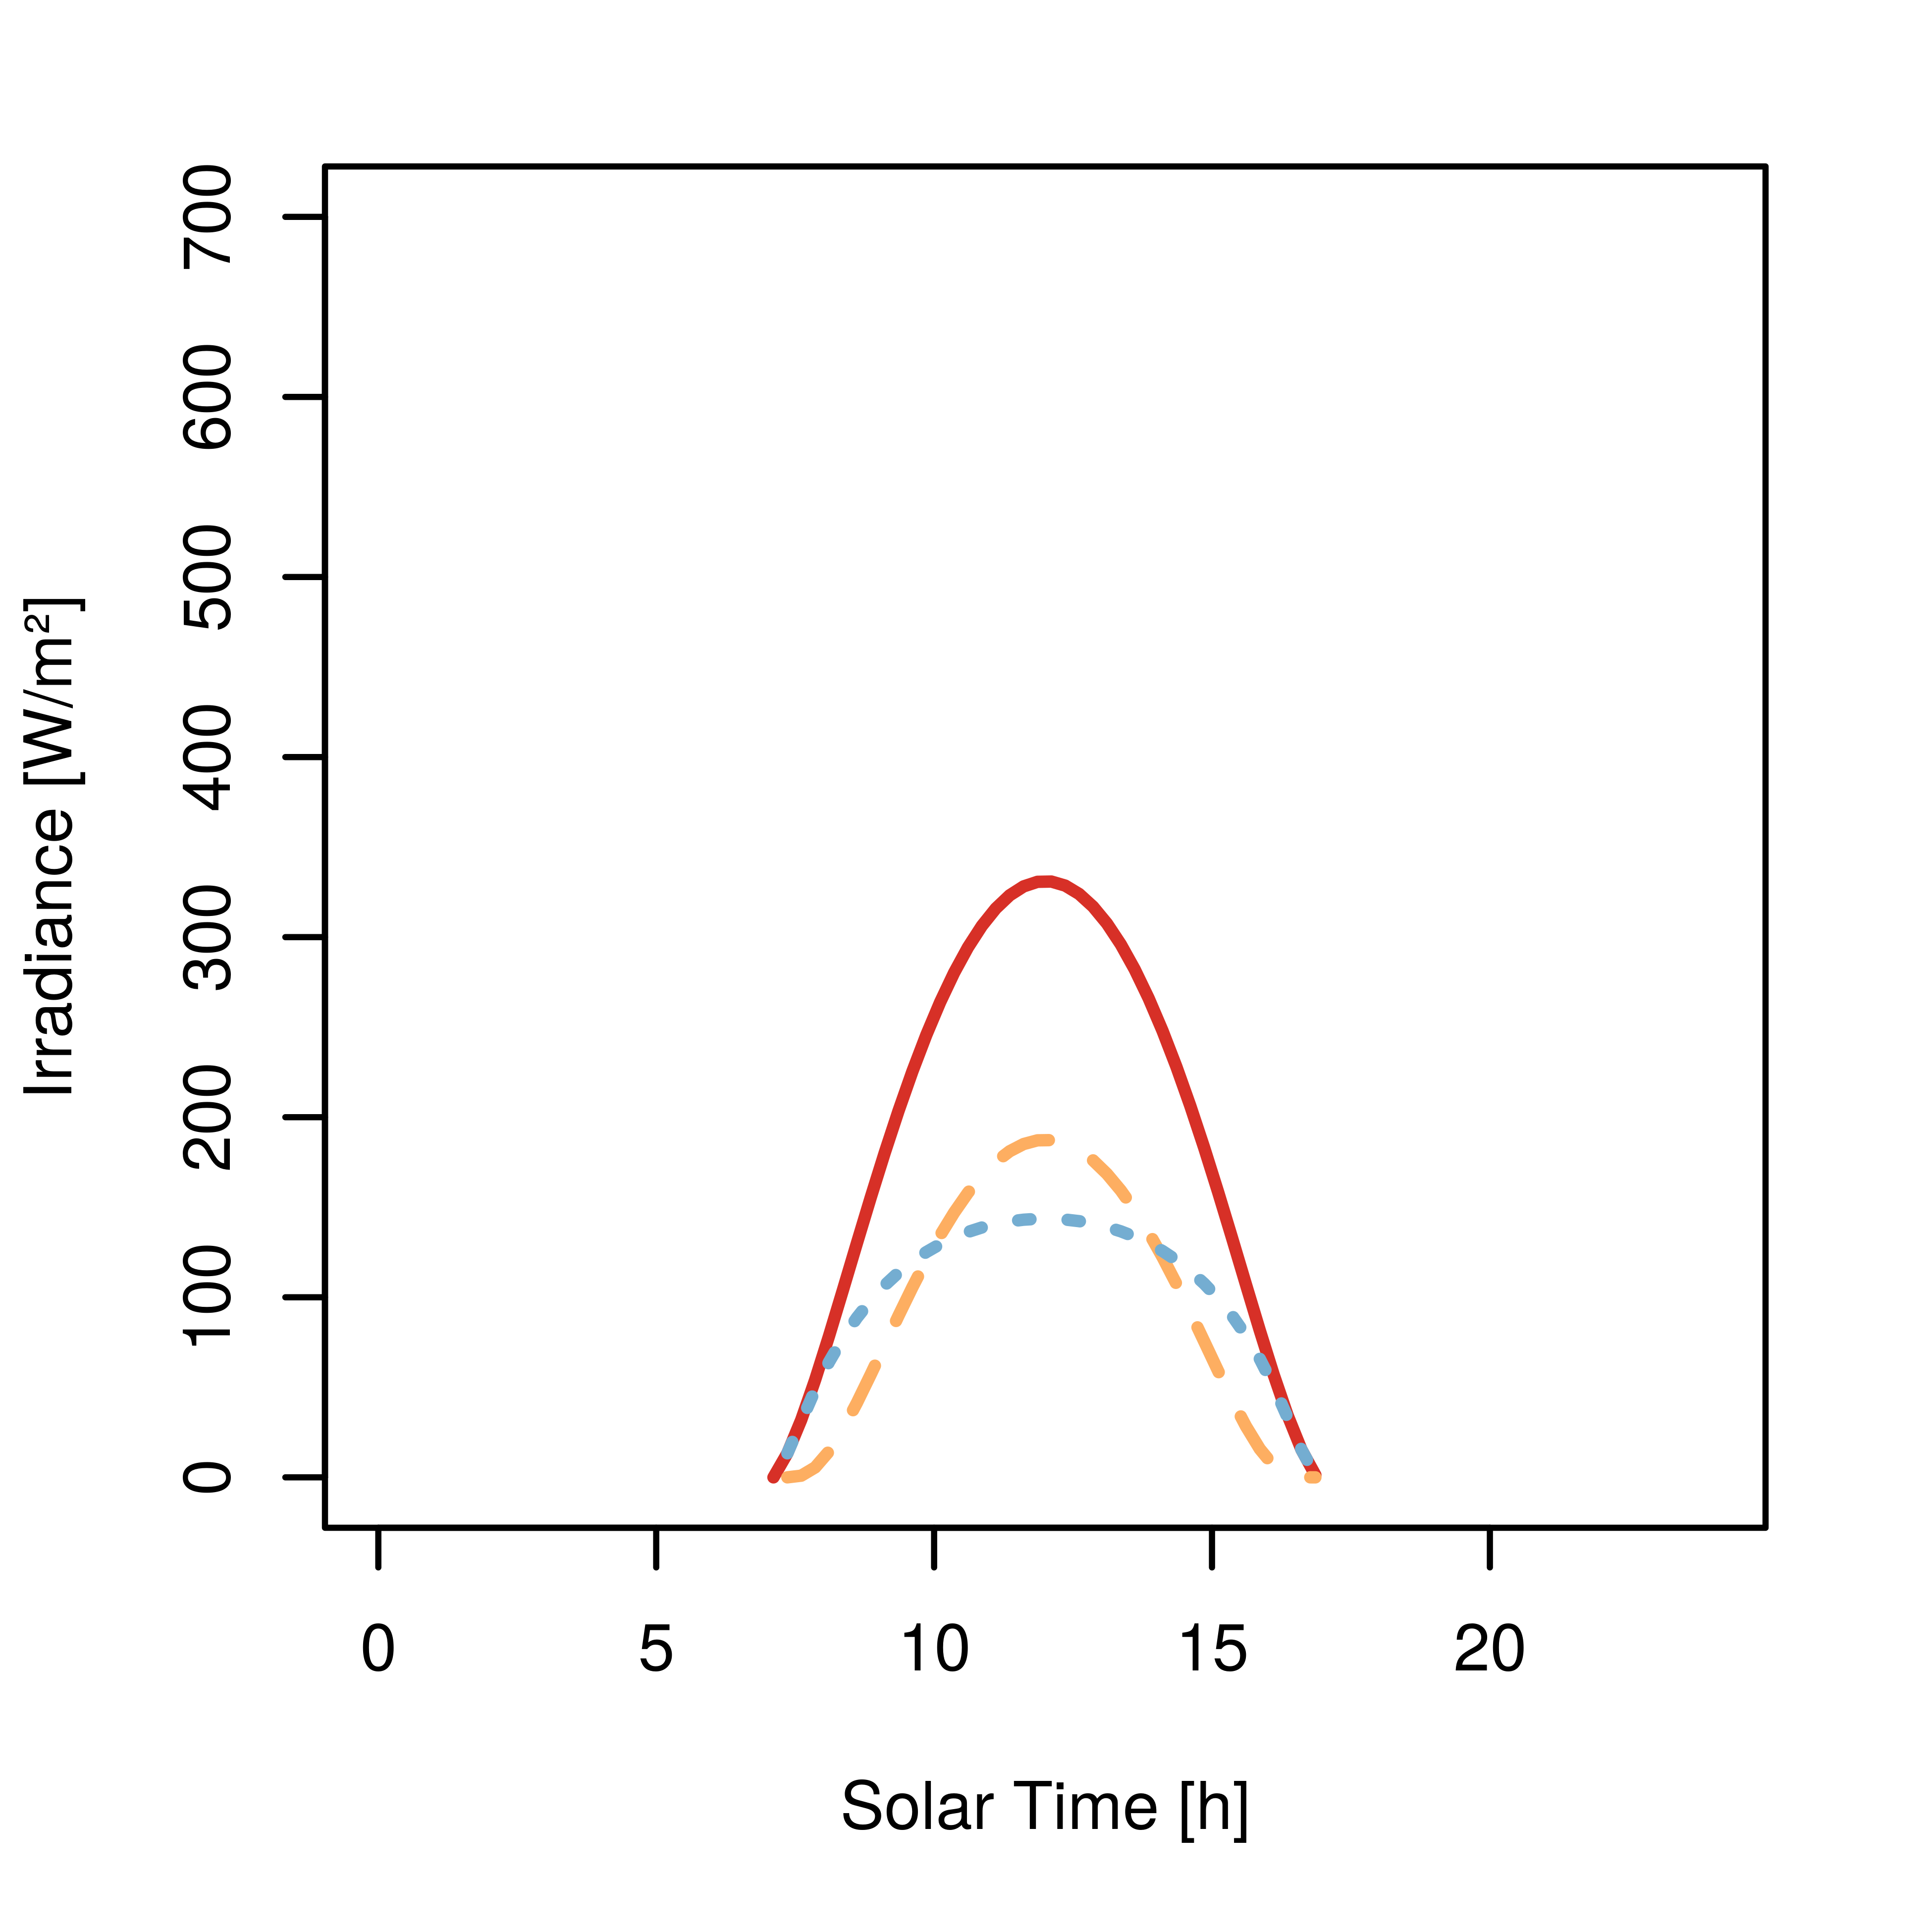
\includegraphics[height=\graphicsHeight]{sections/mars-solar-energy/solar-radiation/plots/gh-gbh-gdh-variation-2-for-ls-248-phi-34-tau-04-and-albedo-027.png}
            \subcaption{$\phi = \SI{34}{\degree}$}
            \label{fig:plot:sub:irradiance-phi-p34}
    \end{subfigure}\\[0.8ex]
    \caption[Diurnal irradiance variations]
    {Diurnal variations of global, beam, and diffuse irradiance on Mars horizontal surface at (a) southern and (b) nothern hemispheres. $L_{s} = \SI{248}{\degree}$ and $\tau = 0.4$.}
    \label{fig:plot:irradiances-phi}
\vspace{-2ex}
\end{figure}

\subsubsection{Insolation}
\label{sec:MartianEnvironment:SolarRadiation:Insolation}

Solar insolation is the amount of solar radiation incident on a surface for a given time period. It is expressed in \si{Whm^{-2}} and obtained by integrating the equations of irradiance over a time period between $\omega_1$ and $\omega_2$. Thus, insolation on a horizontal surface at the top of Mars atmosphere, denoted as $I_{obh}$, is obtained by integrating \refEqn{eq:G_h_2} of $G_{obh}$.


\begin{figure}[h]
\captionsetup[subfigure]{justification=centering}
\vspace{-2ex}
	\centering
    %% setup sizes
    \setlength{\subfigureWidth}{0.50\textwidth}
    \setlength{\graphicsHeight}{70mm}
    %% kill hyper-link highlighting
    \hypersetup{hidelinks=true}%
    %% the figures
%% 1st row
  	\begin{subfigure}[t]{\subfigureWidth}
      \centering
  		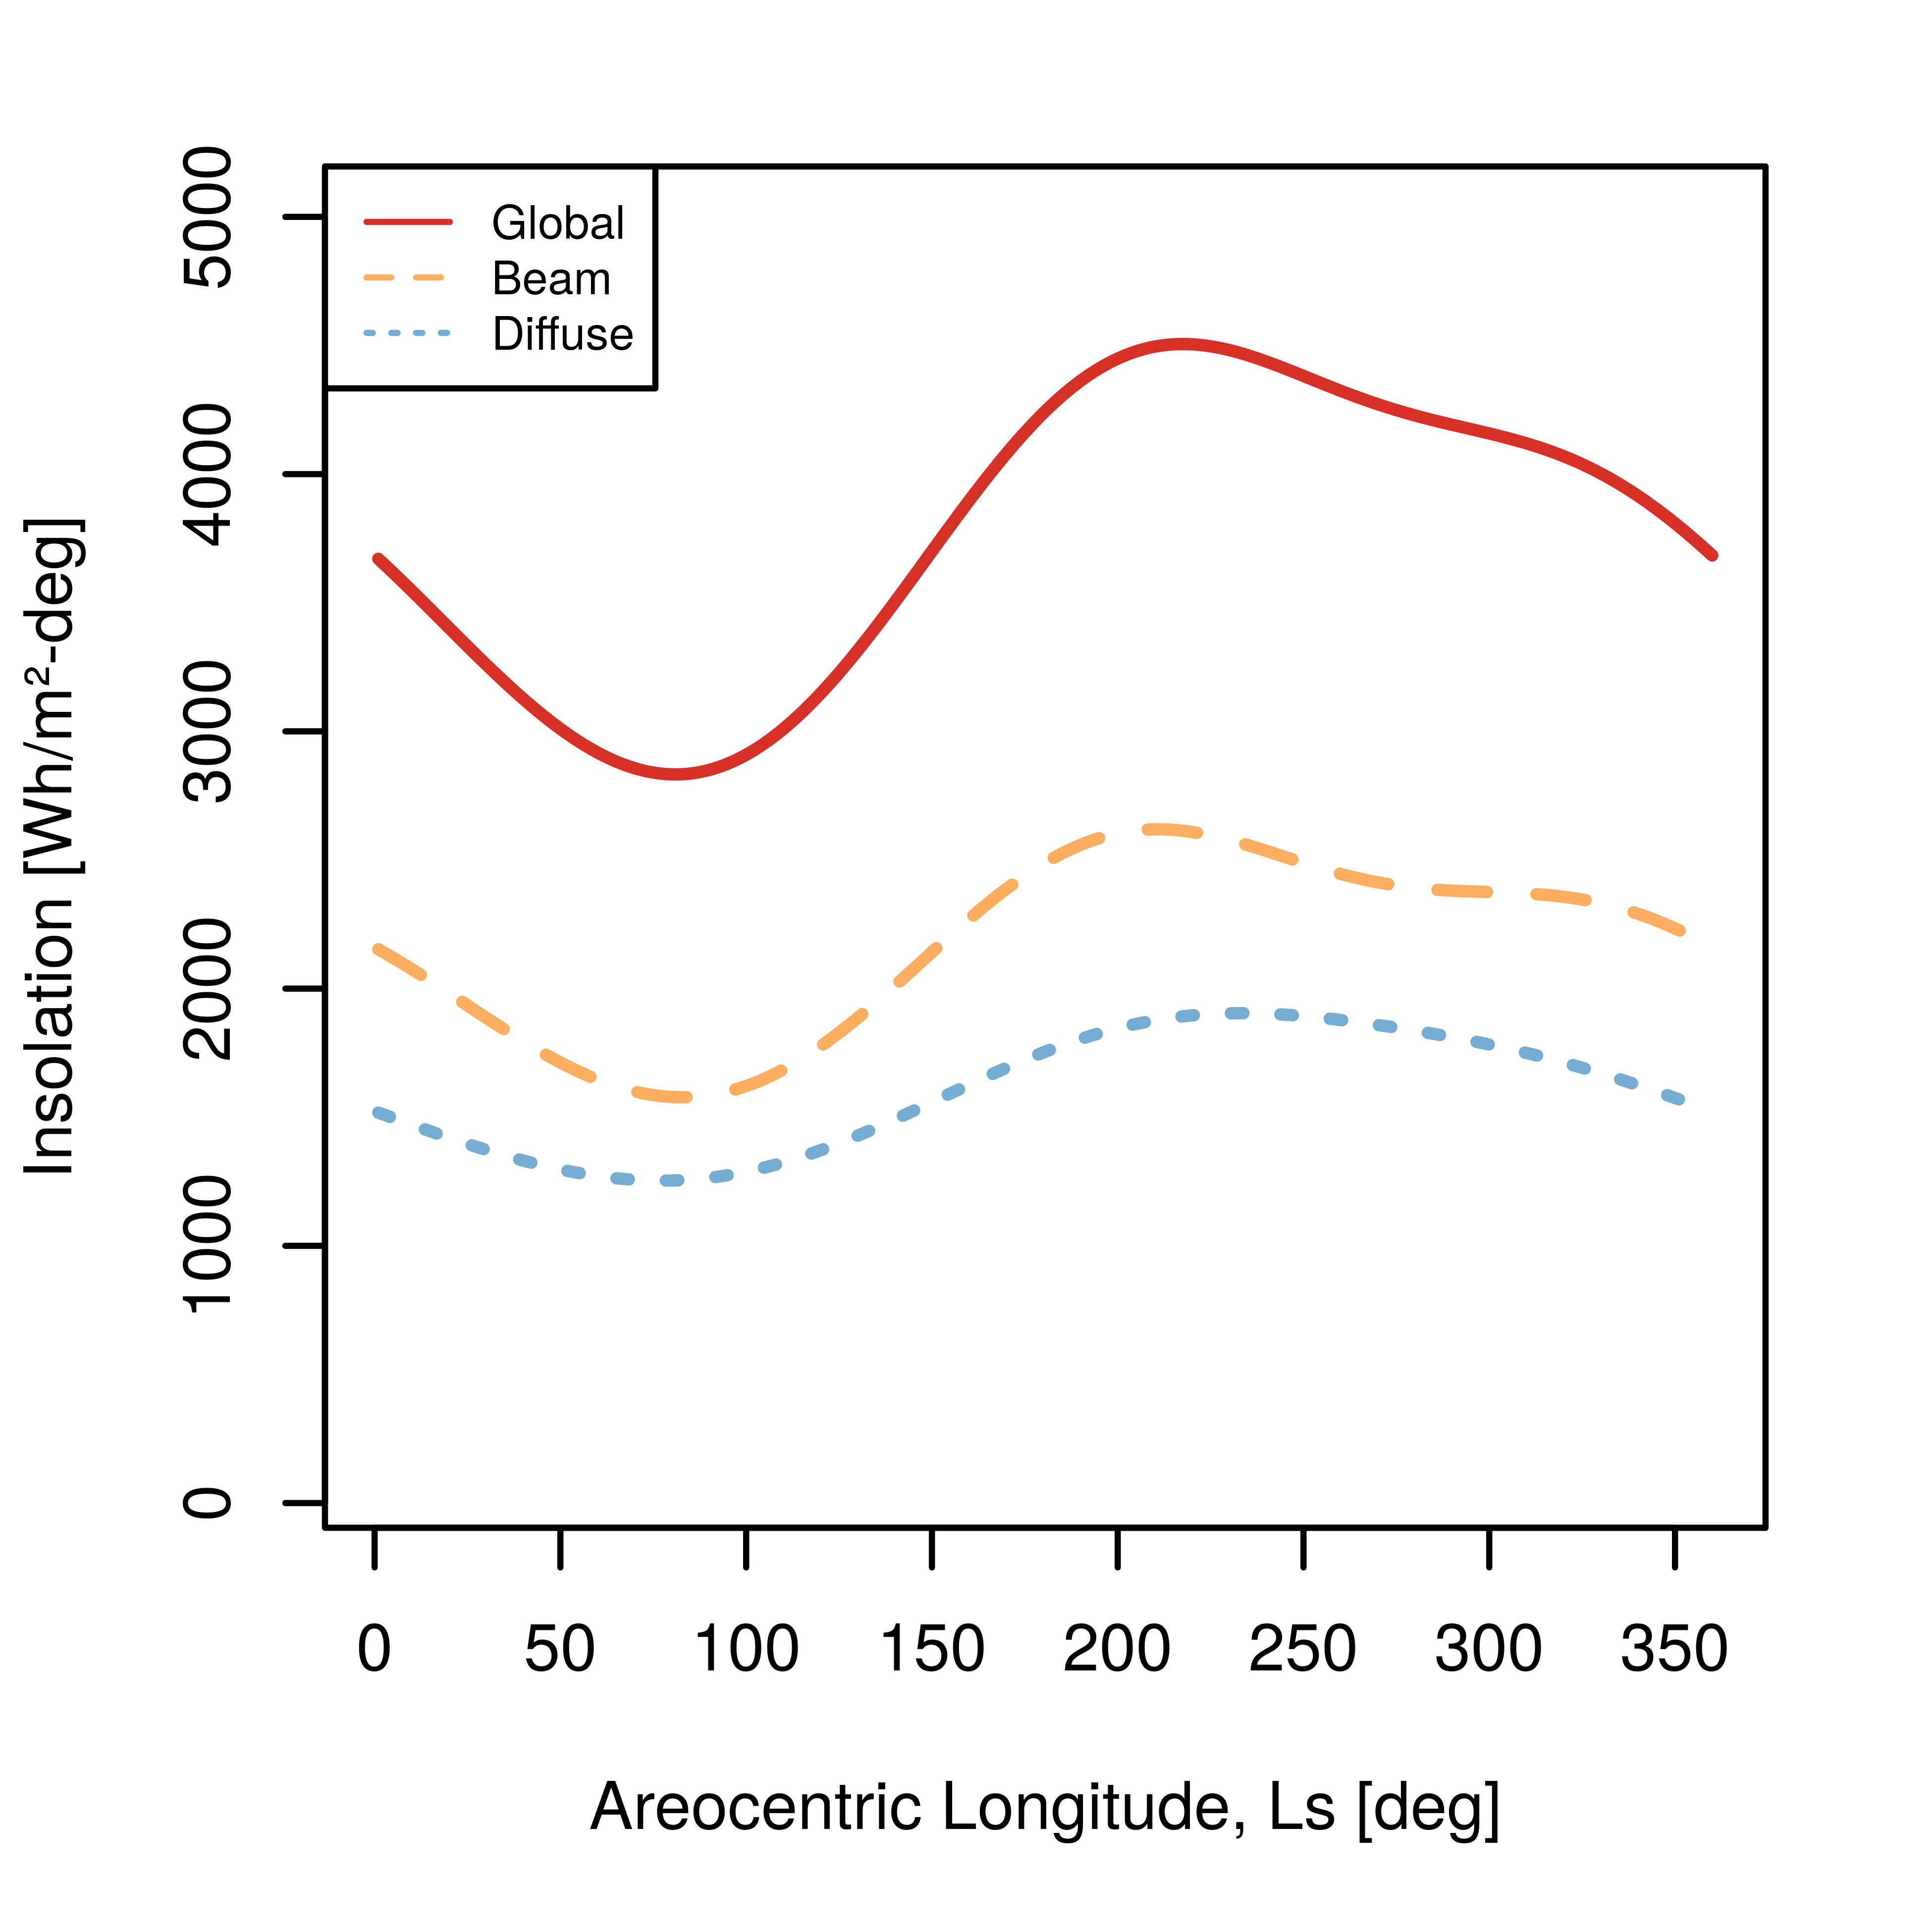
\includegraphics[height=\graphicsHeight]{sections/mars-solar-energy/solar-radiation/plots/hh-hbh-and-hdh-as-a-function-of-ls-for-tau05-phi2-and-albedo-027}
  		\subcaption{$\tau = 0.5$}
  		\label{fig:sub:insolation-ls-tau-factor-0p5}
  	\end{subfigure}\hfill
    \begin{subfigure}[t]{\subfigureWidth}
      \centering
  		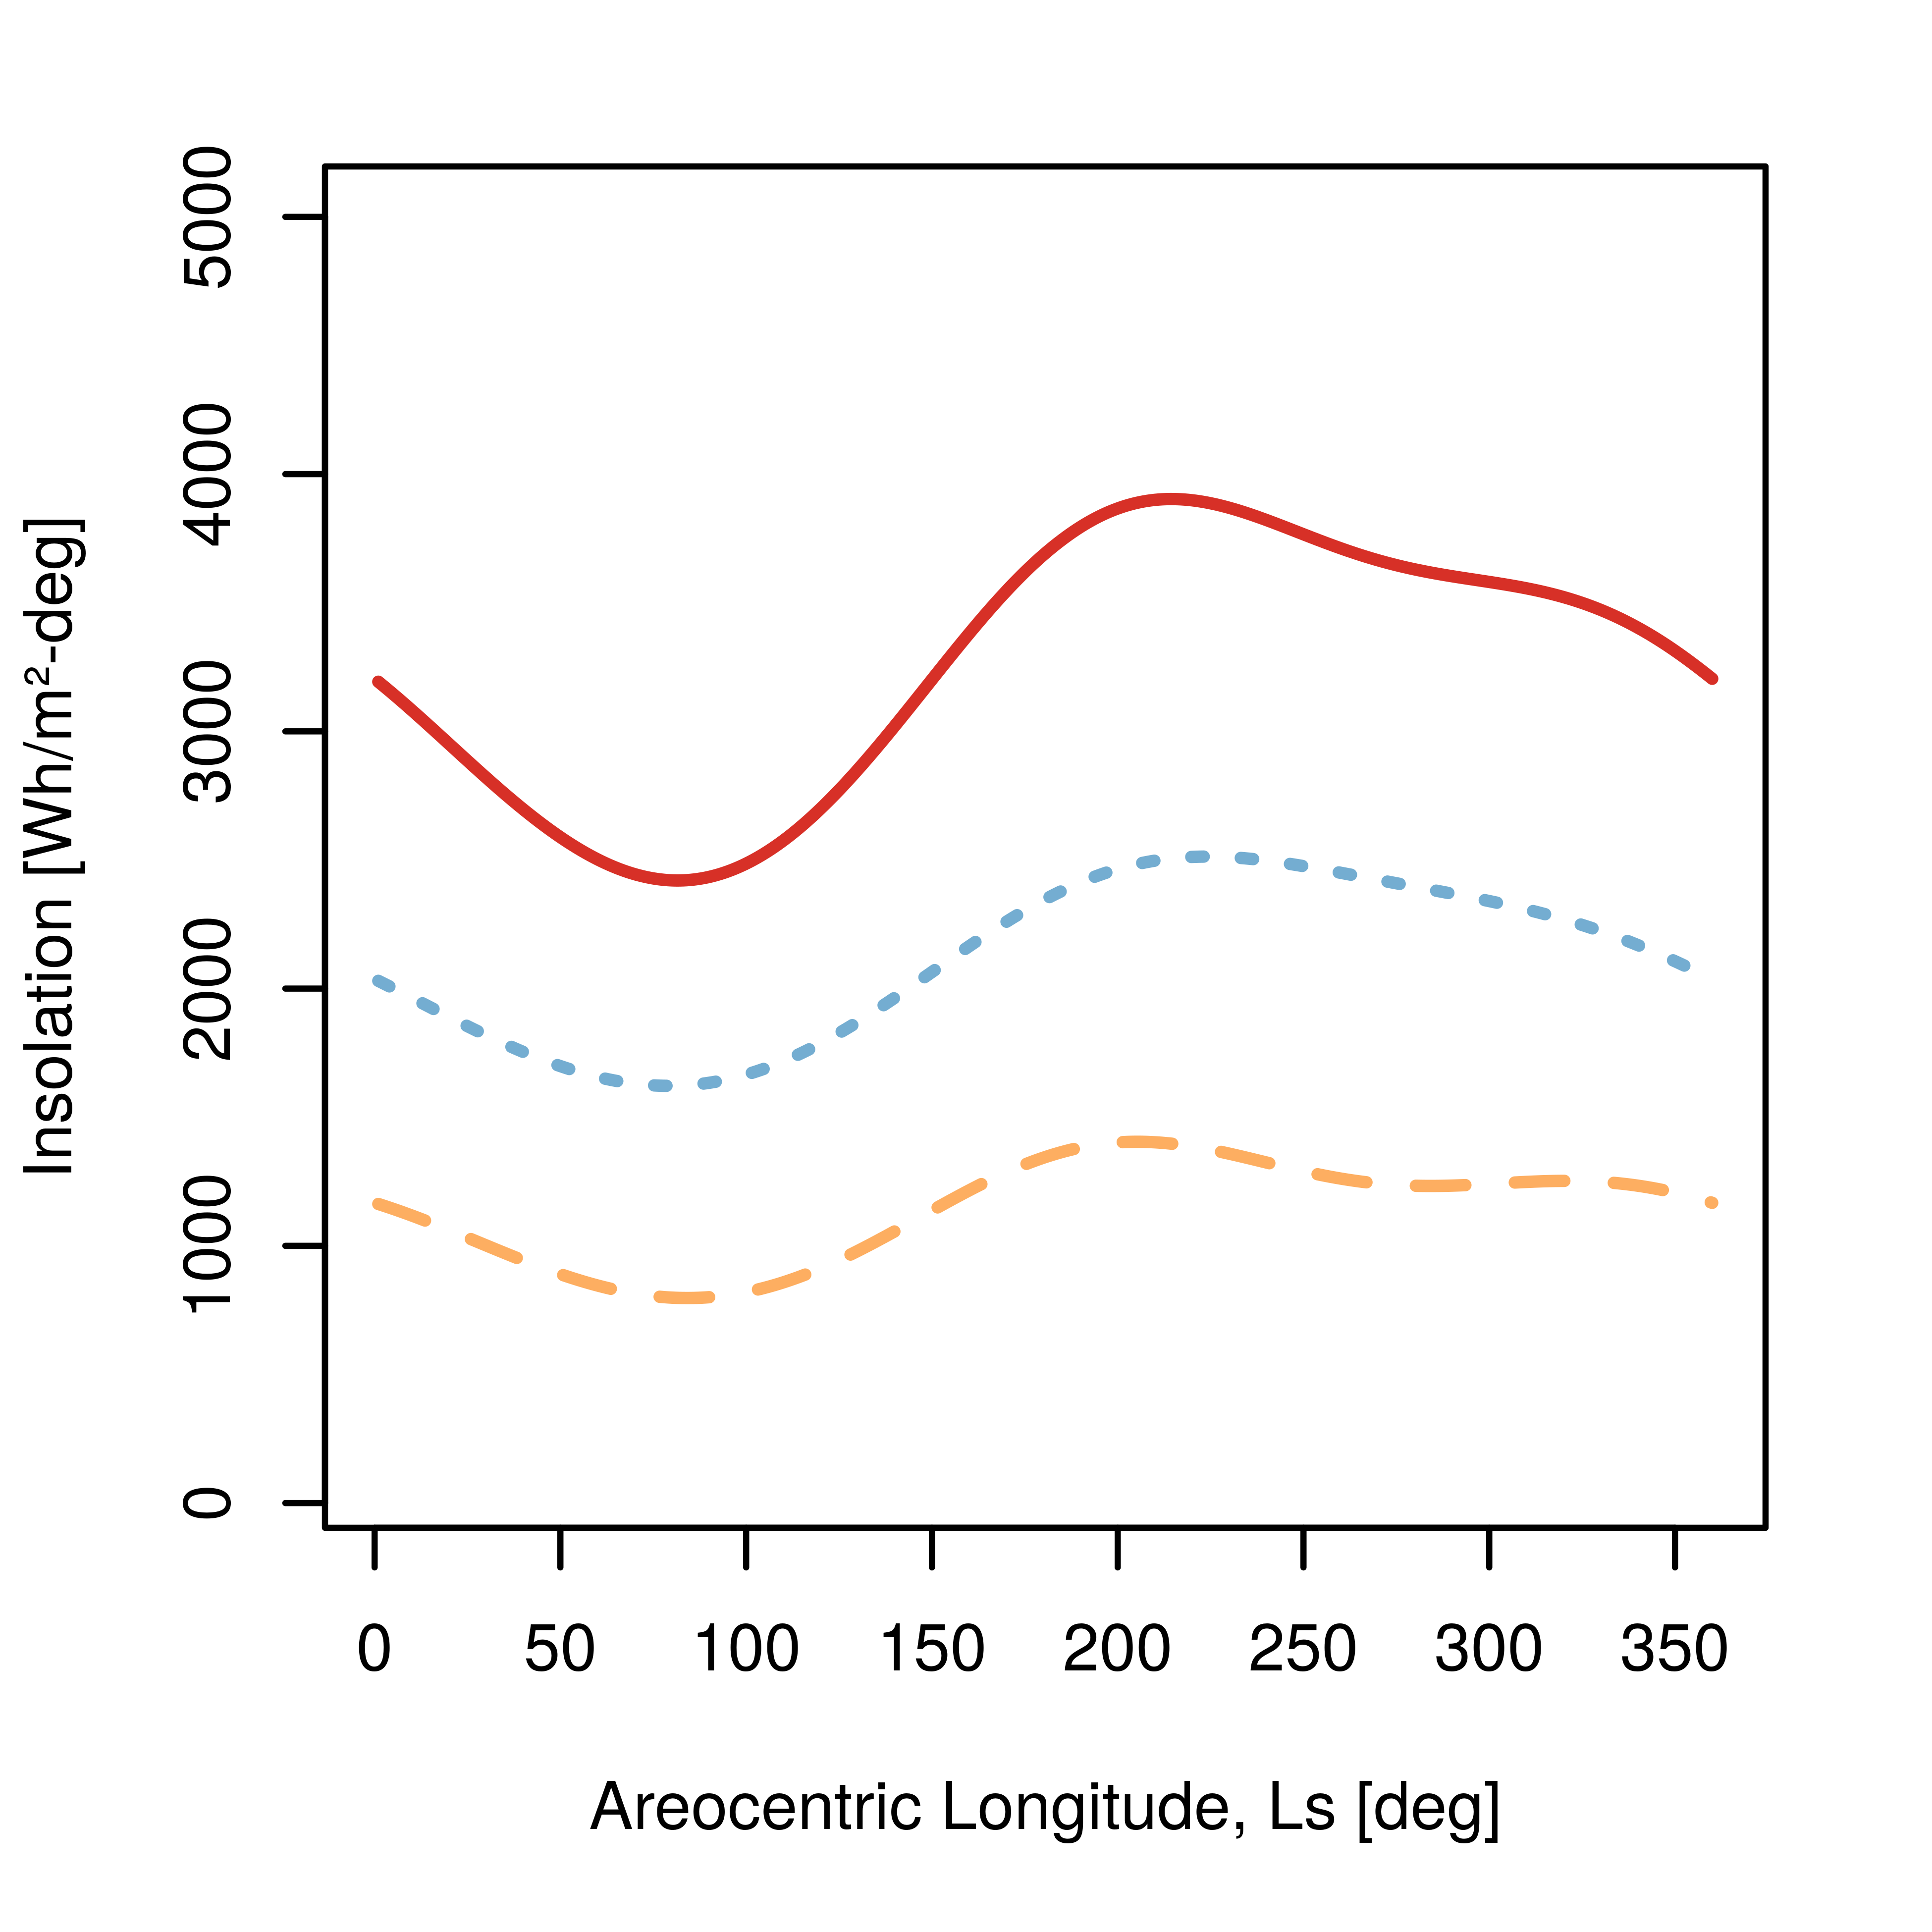
\includegraphics[height=\graphicsHeight]{sections/mars-solar-energy/solar-radiation/plots/hh-hbh-and-hdh-as-a-function-of-ls-for-tau1-phi2-and-albedo-027}
  		\subcaption{$\tau = 1$}
  		\label{fig:sub:insolation-ls-tau-factor-1}
  	\end{subfigure}\\[0.8ex]
%% 2nd row
    \begin{subfigure}[t]{\subfigureWidth}
      \centering
  		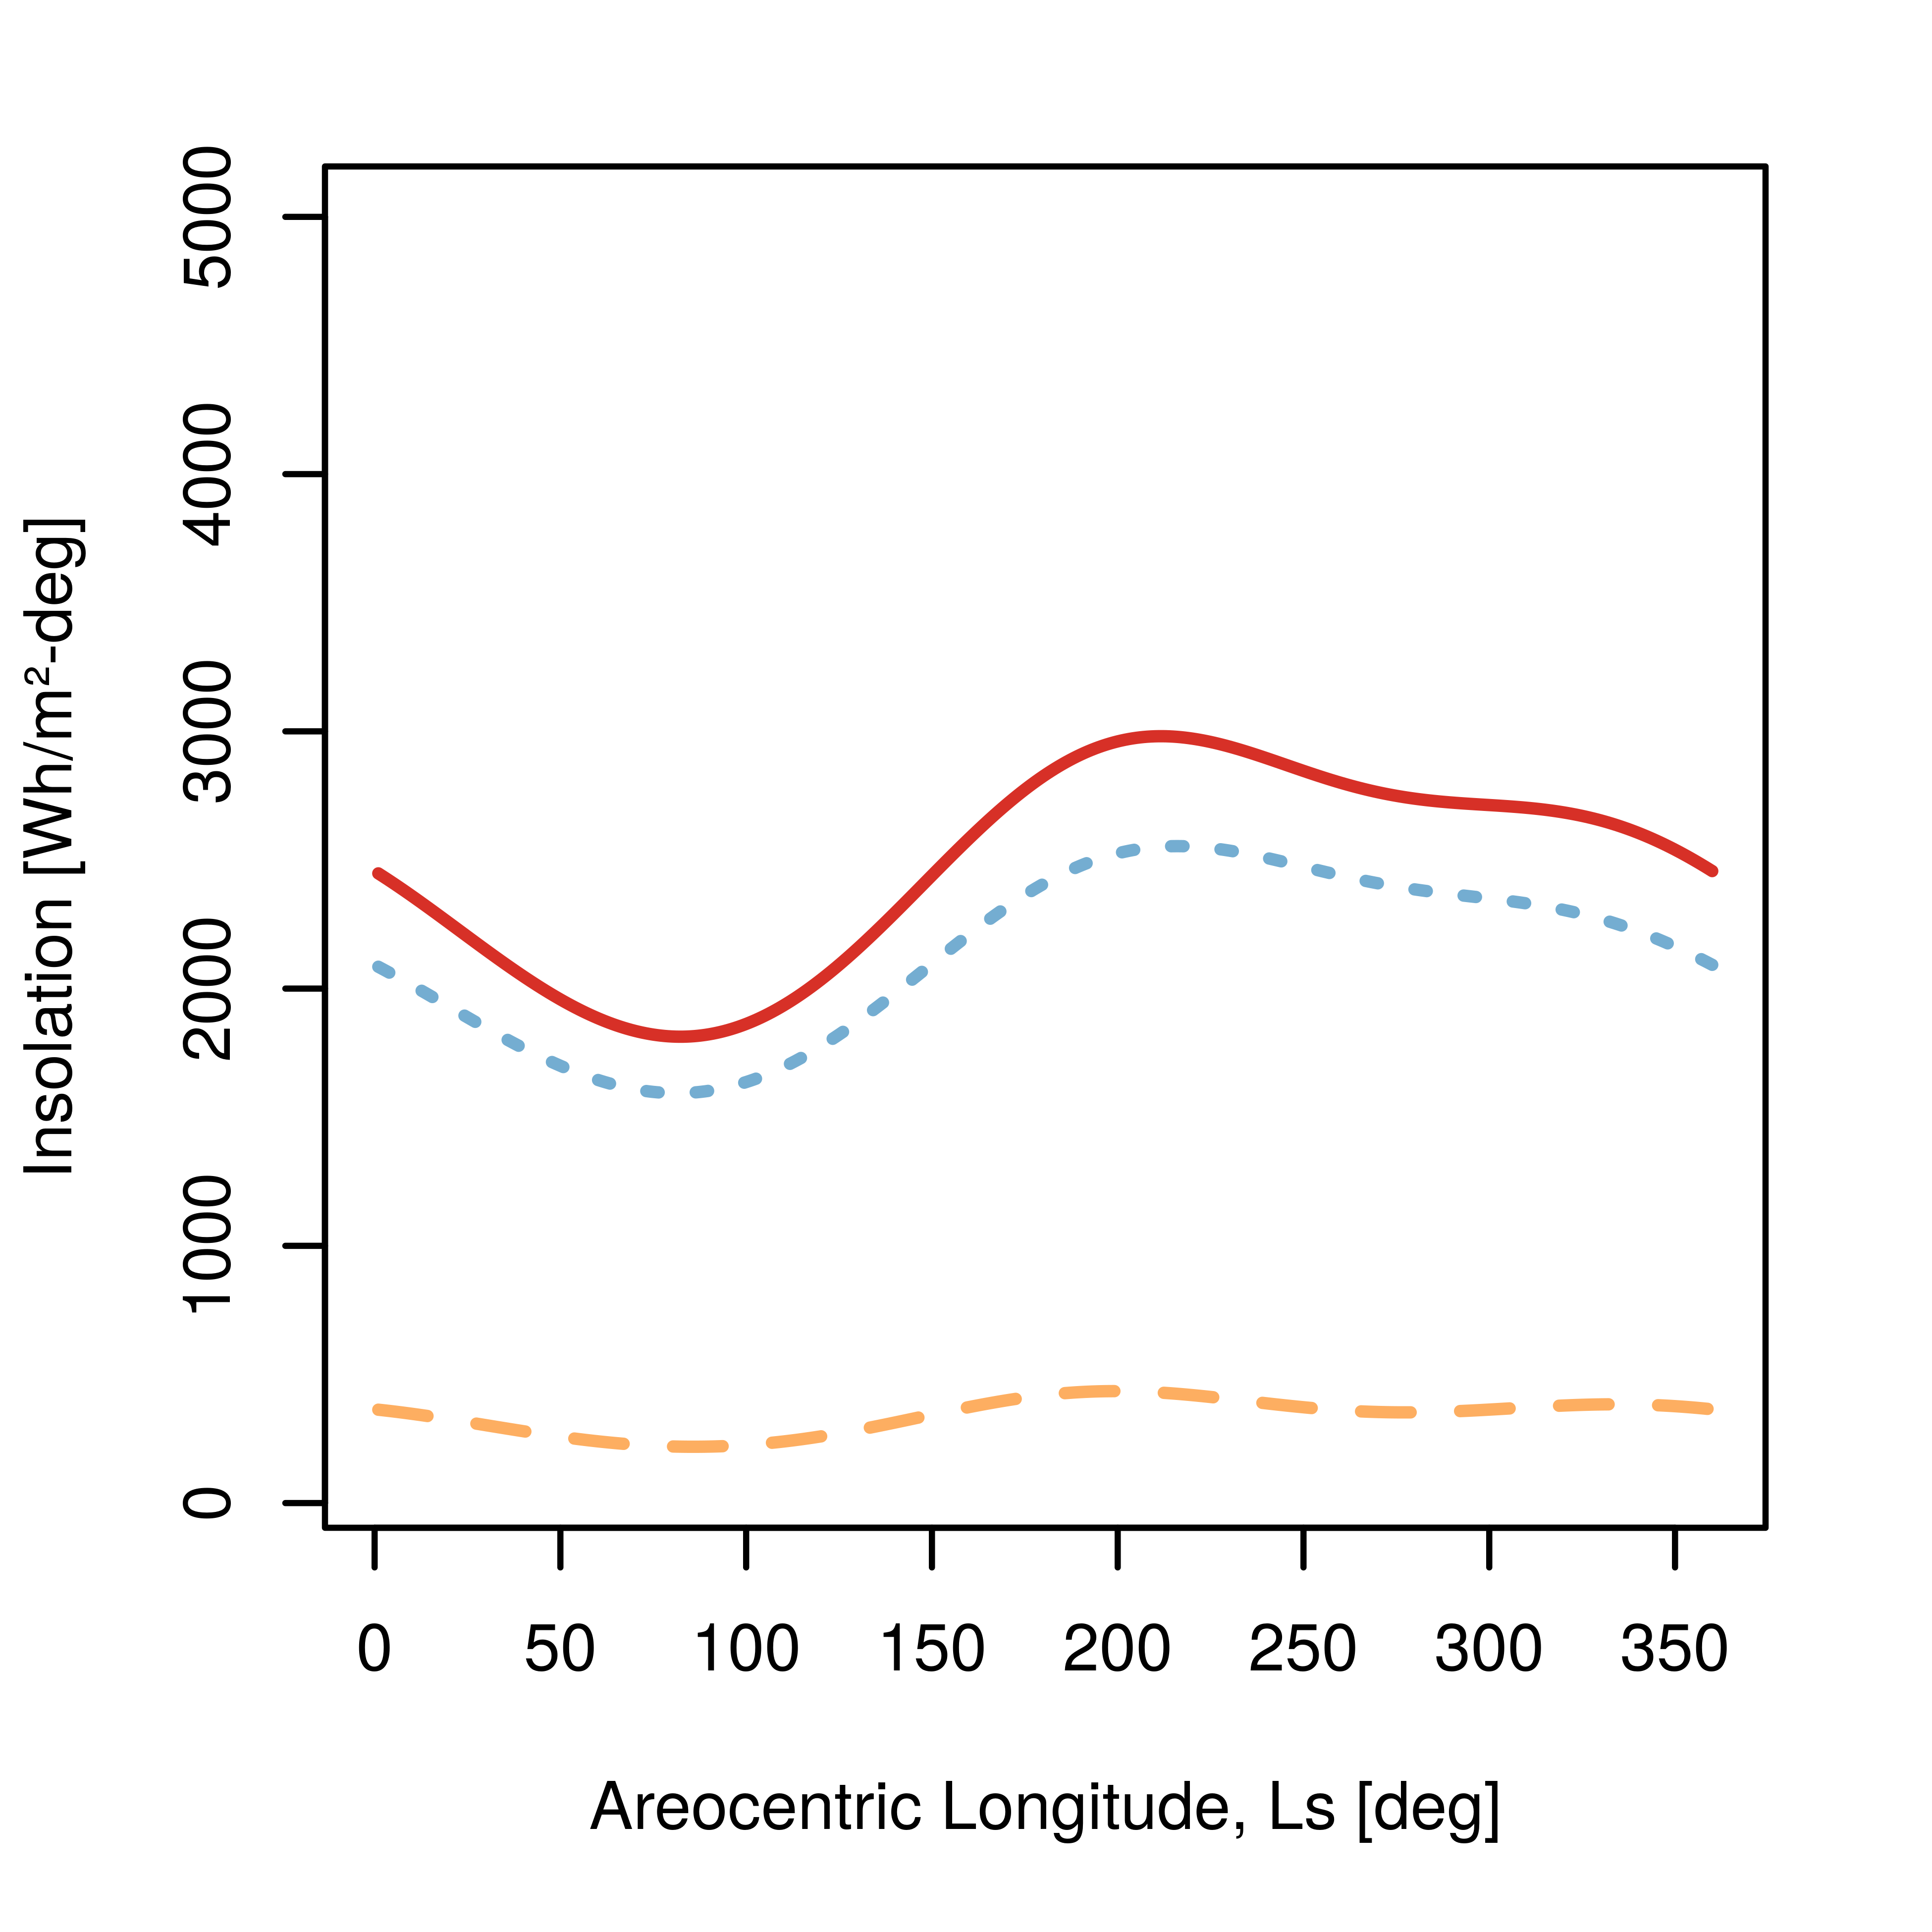
\includegraphics[height=\graphicsHeight]{sections/mars-solar-energy/solar-radiation/plots/hh-hbh-and-hdh-as-a-function-of-ls-for-tau2-phi2-and-albedo-027}
  		\subcaption{$\tau = 2$}
  		\label{fig:sub:insolation-ls-tau-factor-2}
  	\end{subfigure}\hfill
	   \begin{subfigure}[t]{\subfigureWidth}
      \centering
  		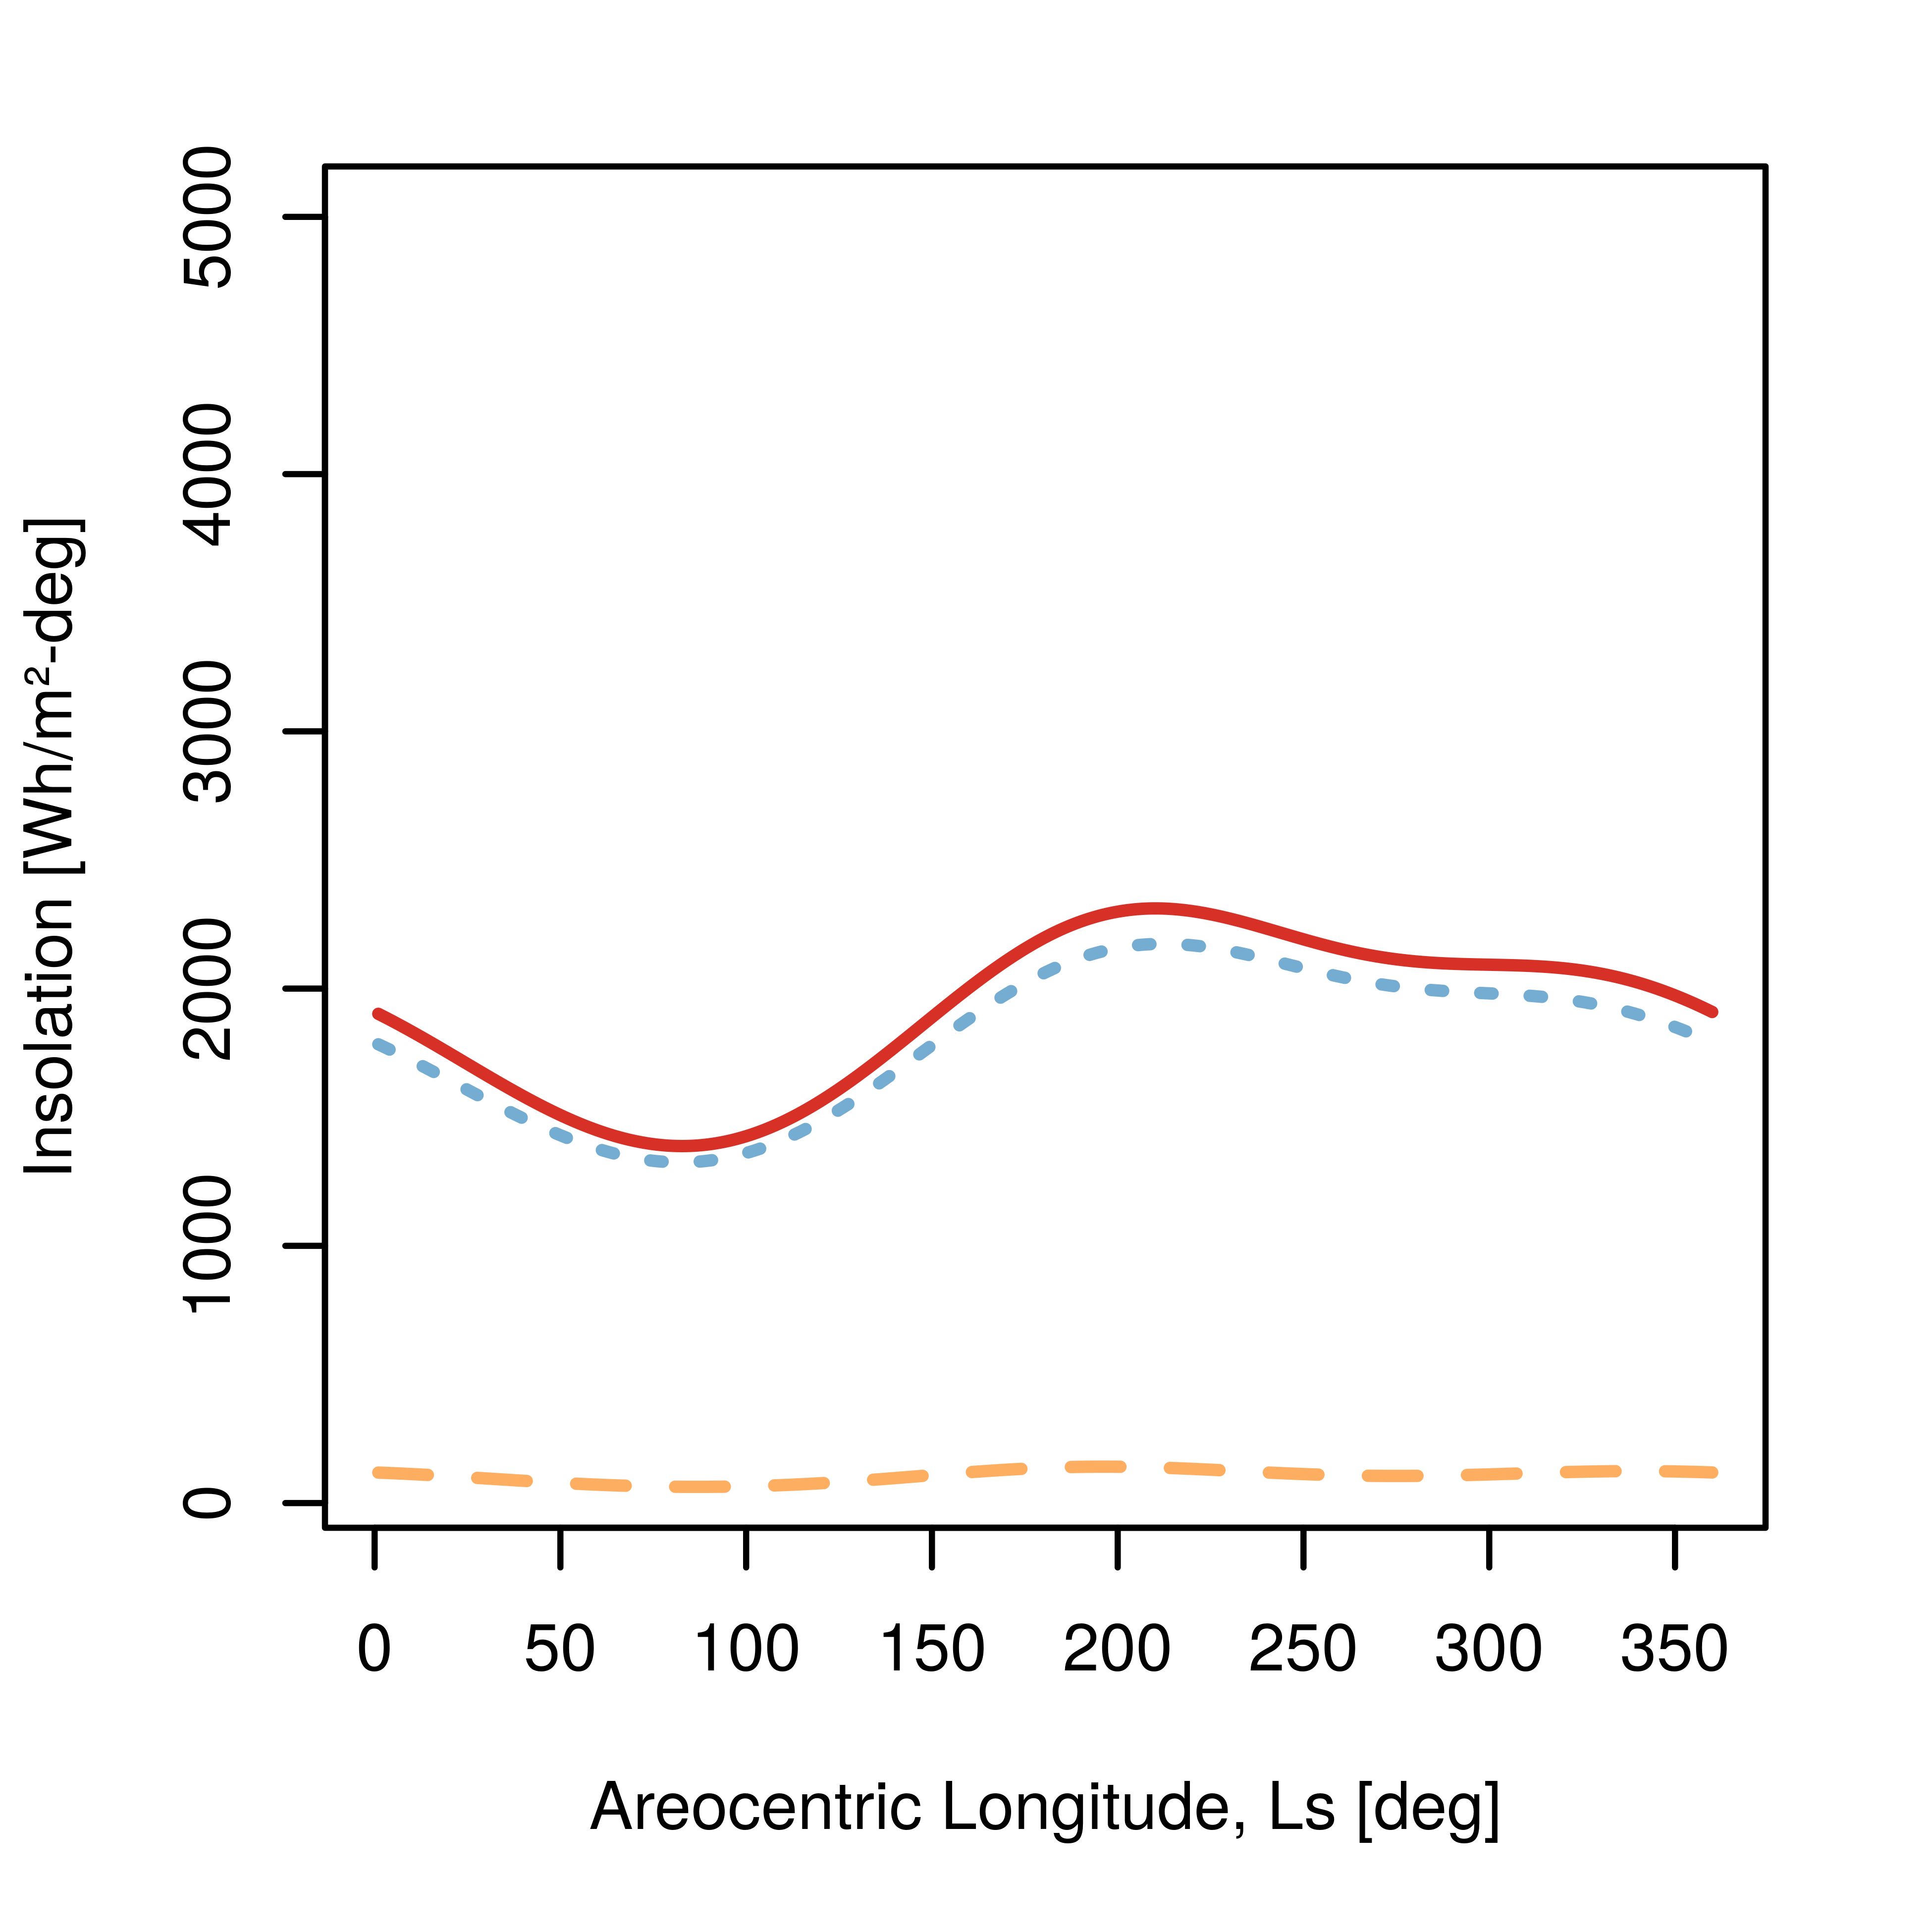
\includegraphics[height=\graphicsHeight]{sections/mars-solar-energy/solar-radiation/plots/hh-hbh-and-hdh-as-a-function-of-ls-for-tau3-phi2-and-albedo-027}
  		\subcaption{$\tau = 3$}
  		\label{fig:sub:insolation-ls-tau-factor-3}
	   \end{subfigure}\hfill
	\caption[Insolation variations]
    {Diurnal variations of global, beam, and diffuse insolation on Mars horizontal surface as a function of areocentric longitude at $\phi = \SI{-2}{\degree}$.}
	\label{fig:plot:insolation-ls}
\vspace{-2ex}
\end{figure}

Global, beam, and diffuse insolations on a horizontal Mars surface are denoted as $I_{h}$, $I_{bh}$, and $I_{dh}$ respectively. Their values are obtained by integrating \refEqn{eq:G_h_2} for $I_{h}$ and \refEqn{eq:G_bh} for $I_{bh}$. Diffuse insolation $I_{dh}$ is obtained through the same relationship presented in \refEqn{eq:G_h_1}. The variation of insolation as a function of $L_{s}$ for different levels of atmospheric opacities are illustrated in \refFig{fig:plot:insolation-ls}. The insolation curves peak at the perihelion with $L_{s} = \SI{248}{\degree}$ and reach their lowest during the aphelion with $L_{s} = \SI{71}{\degree}$. Due to light scattering by airborn dust \citemarsenv{Merikallio2013}, diffuse insolation is already the largest component contributing to the global insolation at $\tau = 1$. On a dusty day at $\tau = 3$, global insolation is mostly diffuse. Daily insolations are obtained when $\omega_1$ and $\omega_2$ are set for a time period between sunrise and sunset. These are denoted as $H_{h}$, $H_{bh}$, and $H_{dh}$ for global, beam, and diffuse insolations on Mars horizontal surface and $H_{obh}$ for a horizontal surface at the top of Mars atmosphere. Similarly to $I_{dh}$, the daily diffuse insolations $H_{dh}$ is obtained from the relationship presented in \refEqn{eq:G_h_1}.

\vspace{0.5cm}

\begin{figure}[h]
\captionsetup[subfigure]{justification=centering}
\vspace{-2ex}
\centering
    %% setup sizes
    \setlength{\subfigureWidth}{0.50\textwidth}
    \setlength{\graphicsHeight}{80mm}
    %% kill hyper-link highlighting
    \hypersetup{hidelinks=true}%
    %% the figures
    \begin{subfigure}[t]{\subfigureWidth}
        \centering
            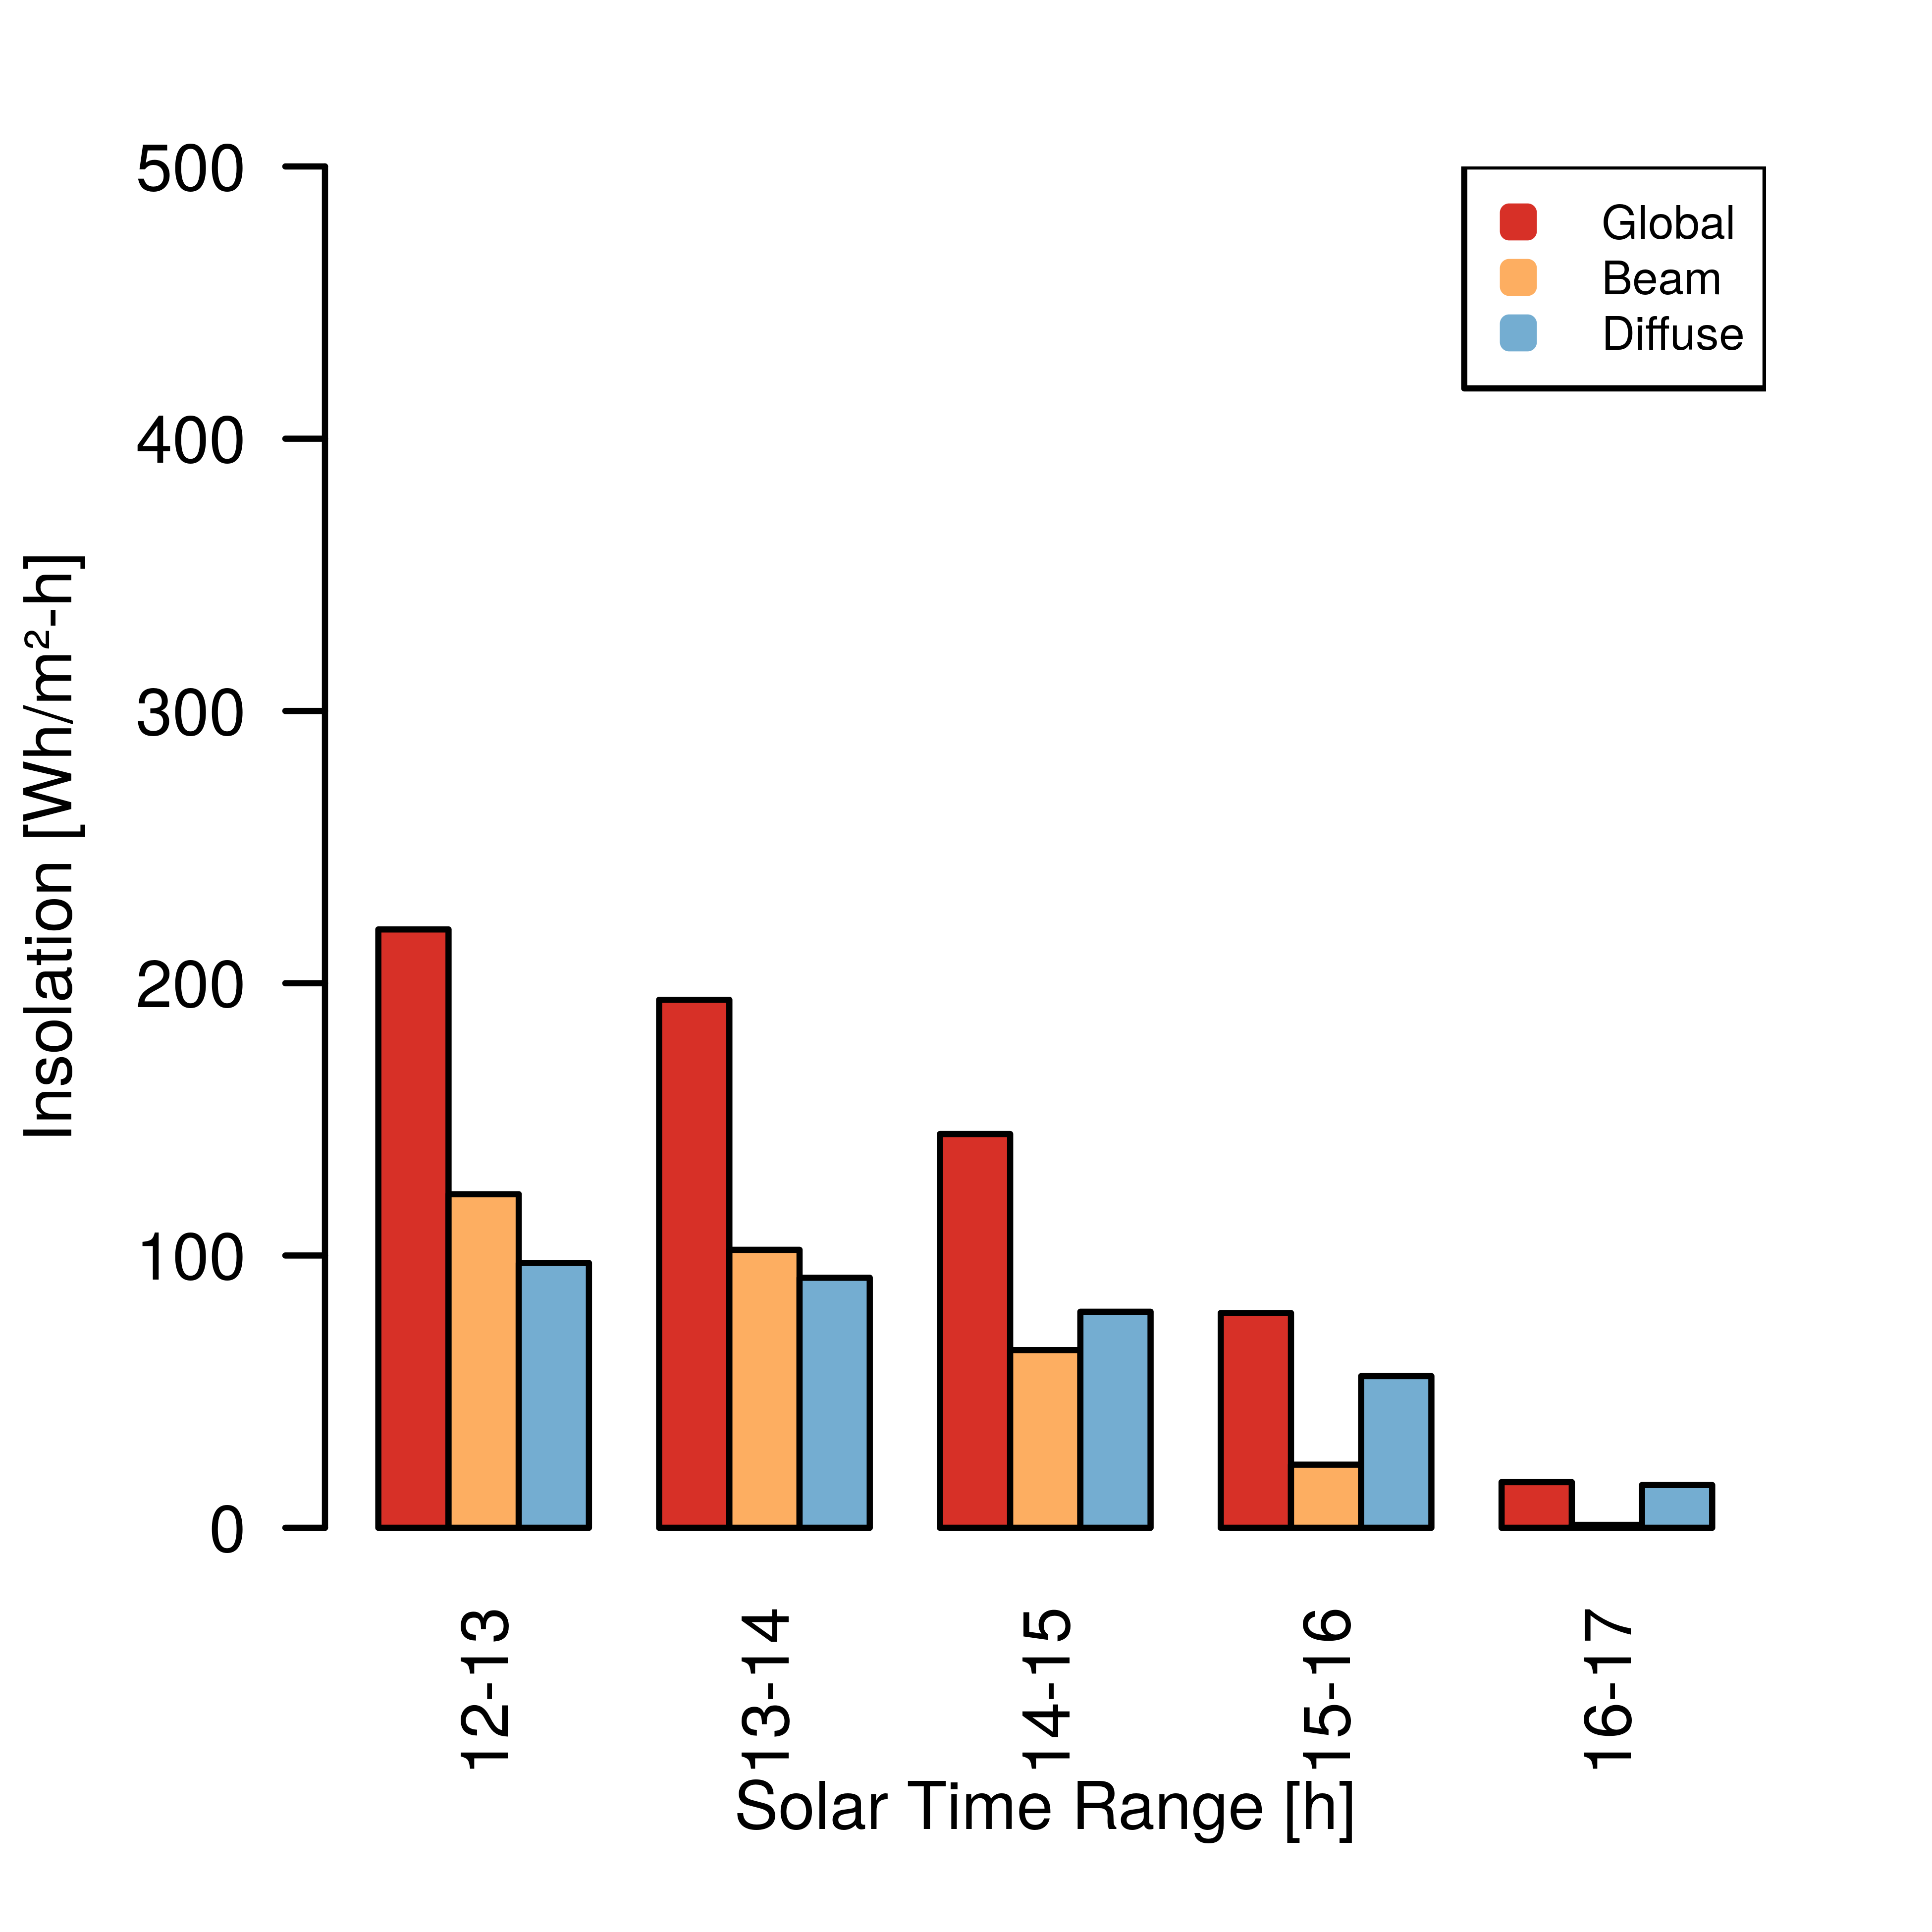
\includegraphics[height=\graphicsHeight]{sections/mars-solar-energy/solar-radiation/plots/ih-ibh-and-idh-variation-1-for-ls-71-phi-34-tau-04-and-albedo-027.png}
            \subcaption{$\phi = \SI{-34}{\degree}$}
            \label{fig:plot:sub:insolation-phi-m34}
    \end{subfigure}\hfill
    \begin{subfigure}[t]{\subfigureWidth}
        \centering
            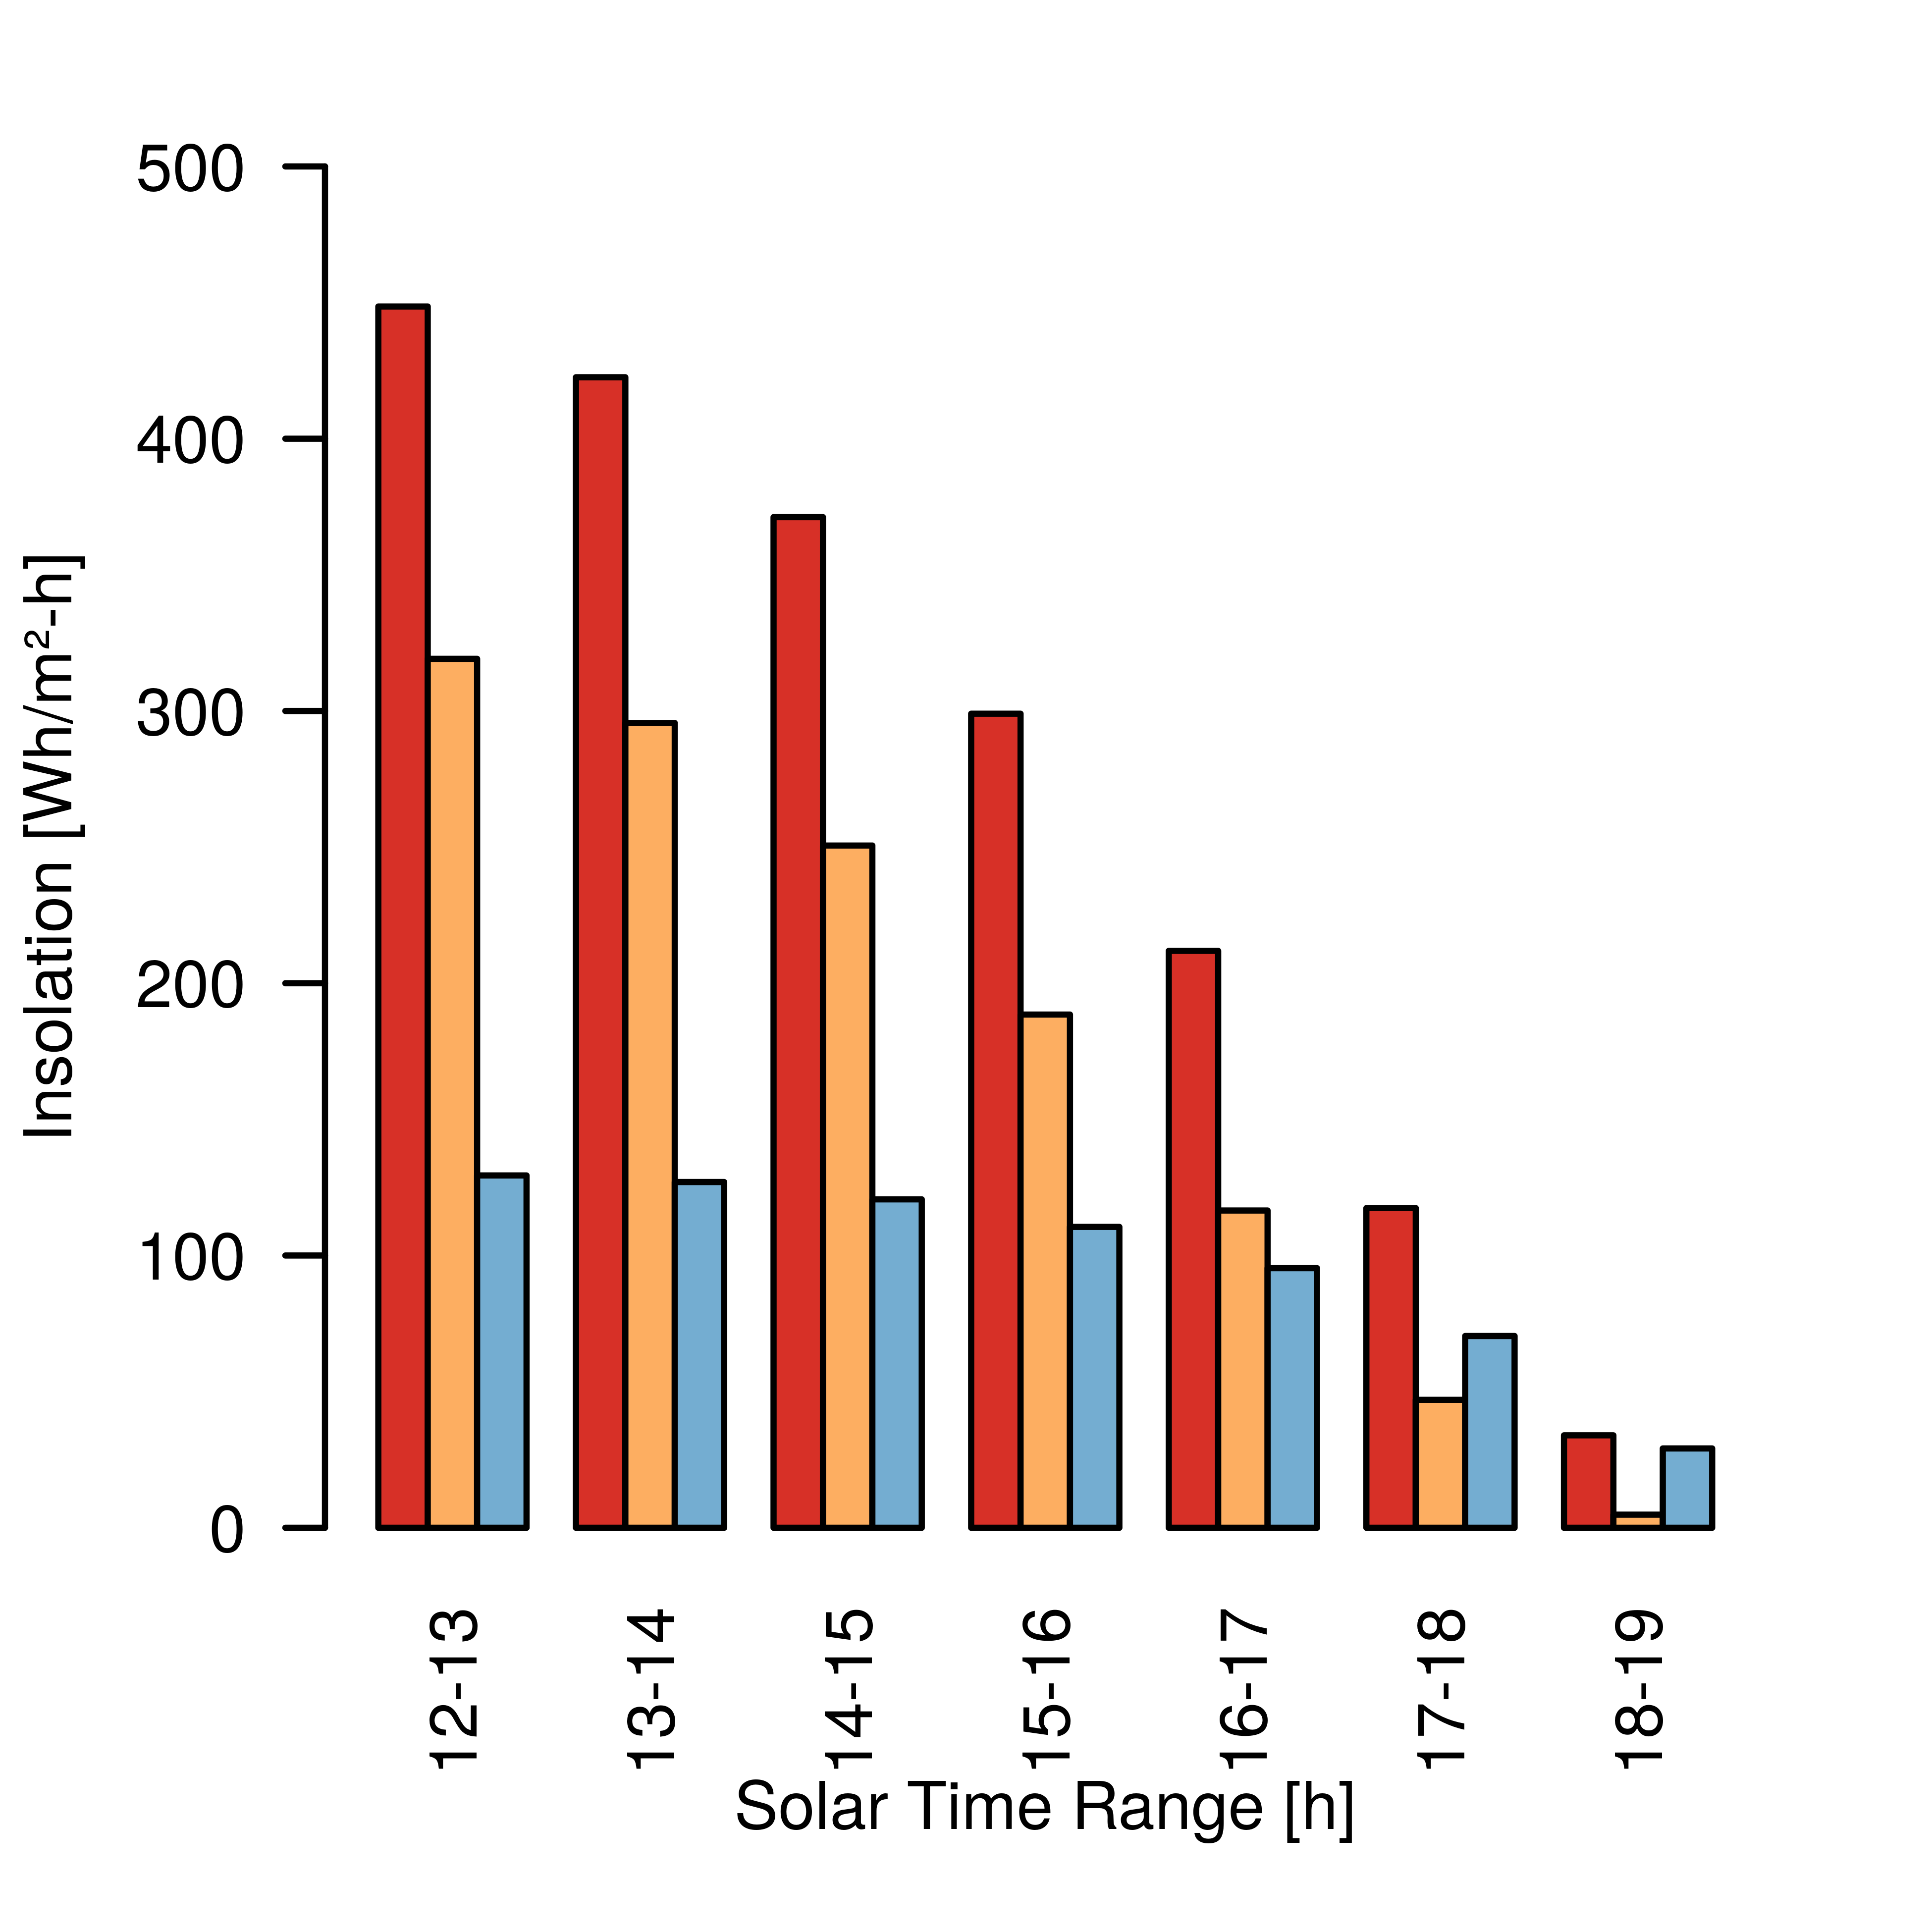
\includegraphics[height=\graphicsHeight]{sections/mars-solar-energy/solar-radiation/plots/ih-ibh-and-idh-variation-2-for-ls-71-phi-34-tau-04-and-albedo-027.png}
            \subcaption{$\phi = \SI{34}{\degree}$}
            \label{fig:plot:sub:insolation-phi-p34}
    \end{subfigure}\\[0.8ex]
    \caption[Diurnal insolation variations]
    {Diurnal variations of global, beam, and diffuse insolation on Mars horizontal surface at (a) southern and (b) nothern hemispheres. Omitted morning insolations are symmetrical to afternoon insolations. $L_{s} = \SI{71}{\degree}$ and $\tau = 0.4$.}
    \label{fig:plot:insolation-phi}
\vspace{-2ex}
\end{figure}

\vspace{0.5cm}

Diurnal profiles are presented in \refFig{fig:plot:insolation-phi} to illustrate insolation variations at the aphelion during a clear Martian day. At $L_{s} = \SI{71}{\degree}$, it is Autumn in the northern hemisphere where insolations are much greater than in the southern hemisphere. Additionally, more daylight is available at \SI{34}{\degree}N than at \SI{34}{\degree}S.

\subsubsection{Inclined Surface}
\label{sec:MartianEnvironment:SolarRadiation:InclinedSurface}

Hitherto the irradiance and insolation calculations on the surface of Mars have been restricted to a horizontal plane. Inclined surfaces are also considered so that \ac{SA} energy production may be maximized during the following cases:
\begin{itemize}
    \item Tilting and orienting the \ac{SA} into optimal inclination and orientation angles while the rover is on a horizontal surface.
    \item Tilting and orienting the \ac{SA} towards a horizontal plane while the rover is on an inclined surface facing away from the Sun.
    \item Traversing descent and ascent profiles such as in the topographic slope variations in a crater exploration mission.
\end{itemize}

\clearpage
Descriptions of the angles involved as well as how they serve to position the \ac{SA} surface are presented in \refApp{sec:Appendix:OptimalAngles}. Global irradiance $G_{\beta}$ on an inclined surface is obtained when parametizing the inclination angle $\beta$ and the Sun angle of incidence $\theta$. This is shown in \refEqn{eq:G_beta}:

\begin{equation}
  \label{eq:G_beta}
  G_{\beta} = G_{b}\cos{(\theta)} + G_{dh}\cos{\left(\frac{\beta}{2}\right)}^2 + al G_{h} \sin{\left(\frac{\beta}{2}\right)}^2
\end{equation}

where $al$ is the albedo. The Sun angle of incidence is obtained with \refEqn{eq:costheta}. It is a function of the Sun zenith angle $z$ for the time of day, the solar azimuth $\gamma_{s}$, the angle $\beta$ for the slope inclination, and the Sun surface azimuth angle $\gamma_{c}$ for the orientation that the inclination is facing.

\begin{equation}
  \label{eq:costheta}
  \cos{(\theta)} = \cos{(\beta)}\cos{(z)} + \sin{(\beta)}\sin{(z)}\cos{(\gamma_{s} - \gamma_{c})}
\end{equation}

\begin{figure}[h]
\captionsetup[subfigure]{justification=centering}
\vspace{-2ex}
	\centering
    %% setup sizes
    \setlength{\subfigureWidth}{0.50\textwidth}
    \setlength{\graphicsHeight}{70mm}
    %% kill hyper-link highlighting
    \hypersetup{hidelinks=true}%
    %% the figures
%% 1st row
  	\begin{subfigure}[t]{\subfigureWidth}
      \centering
  		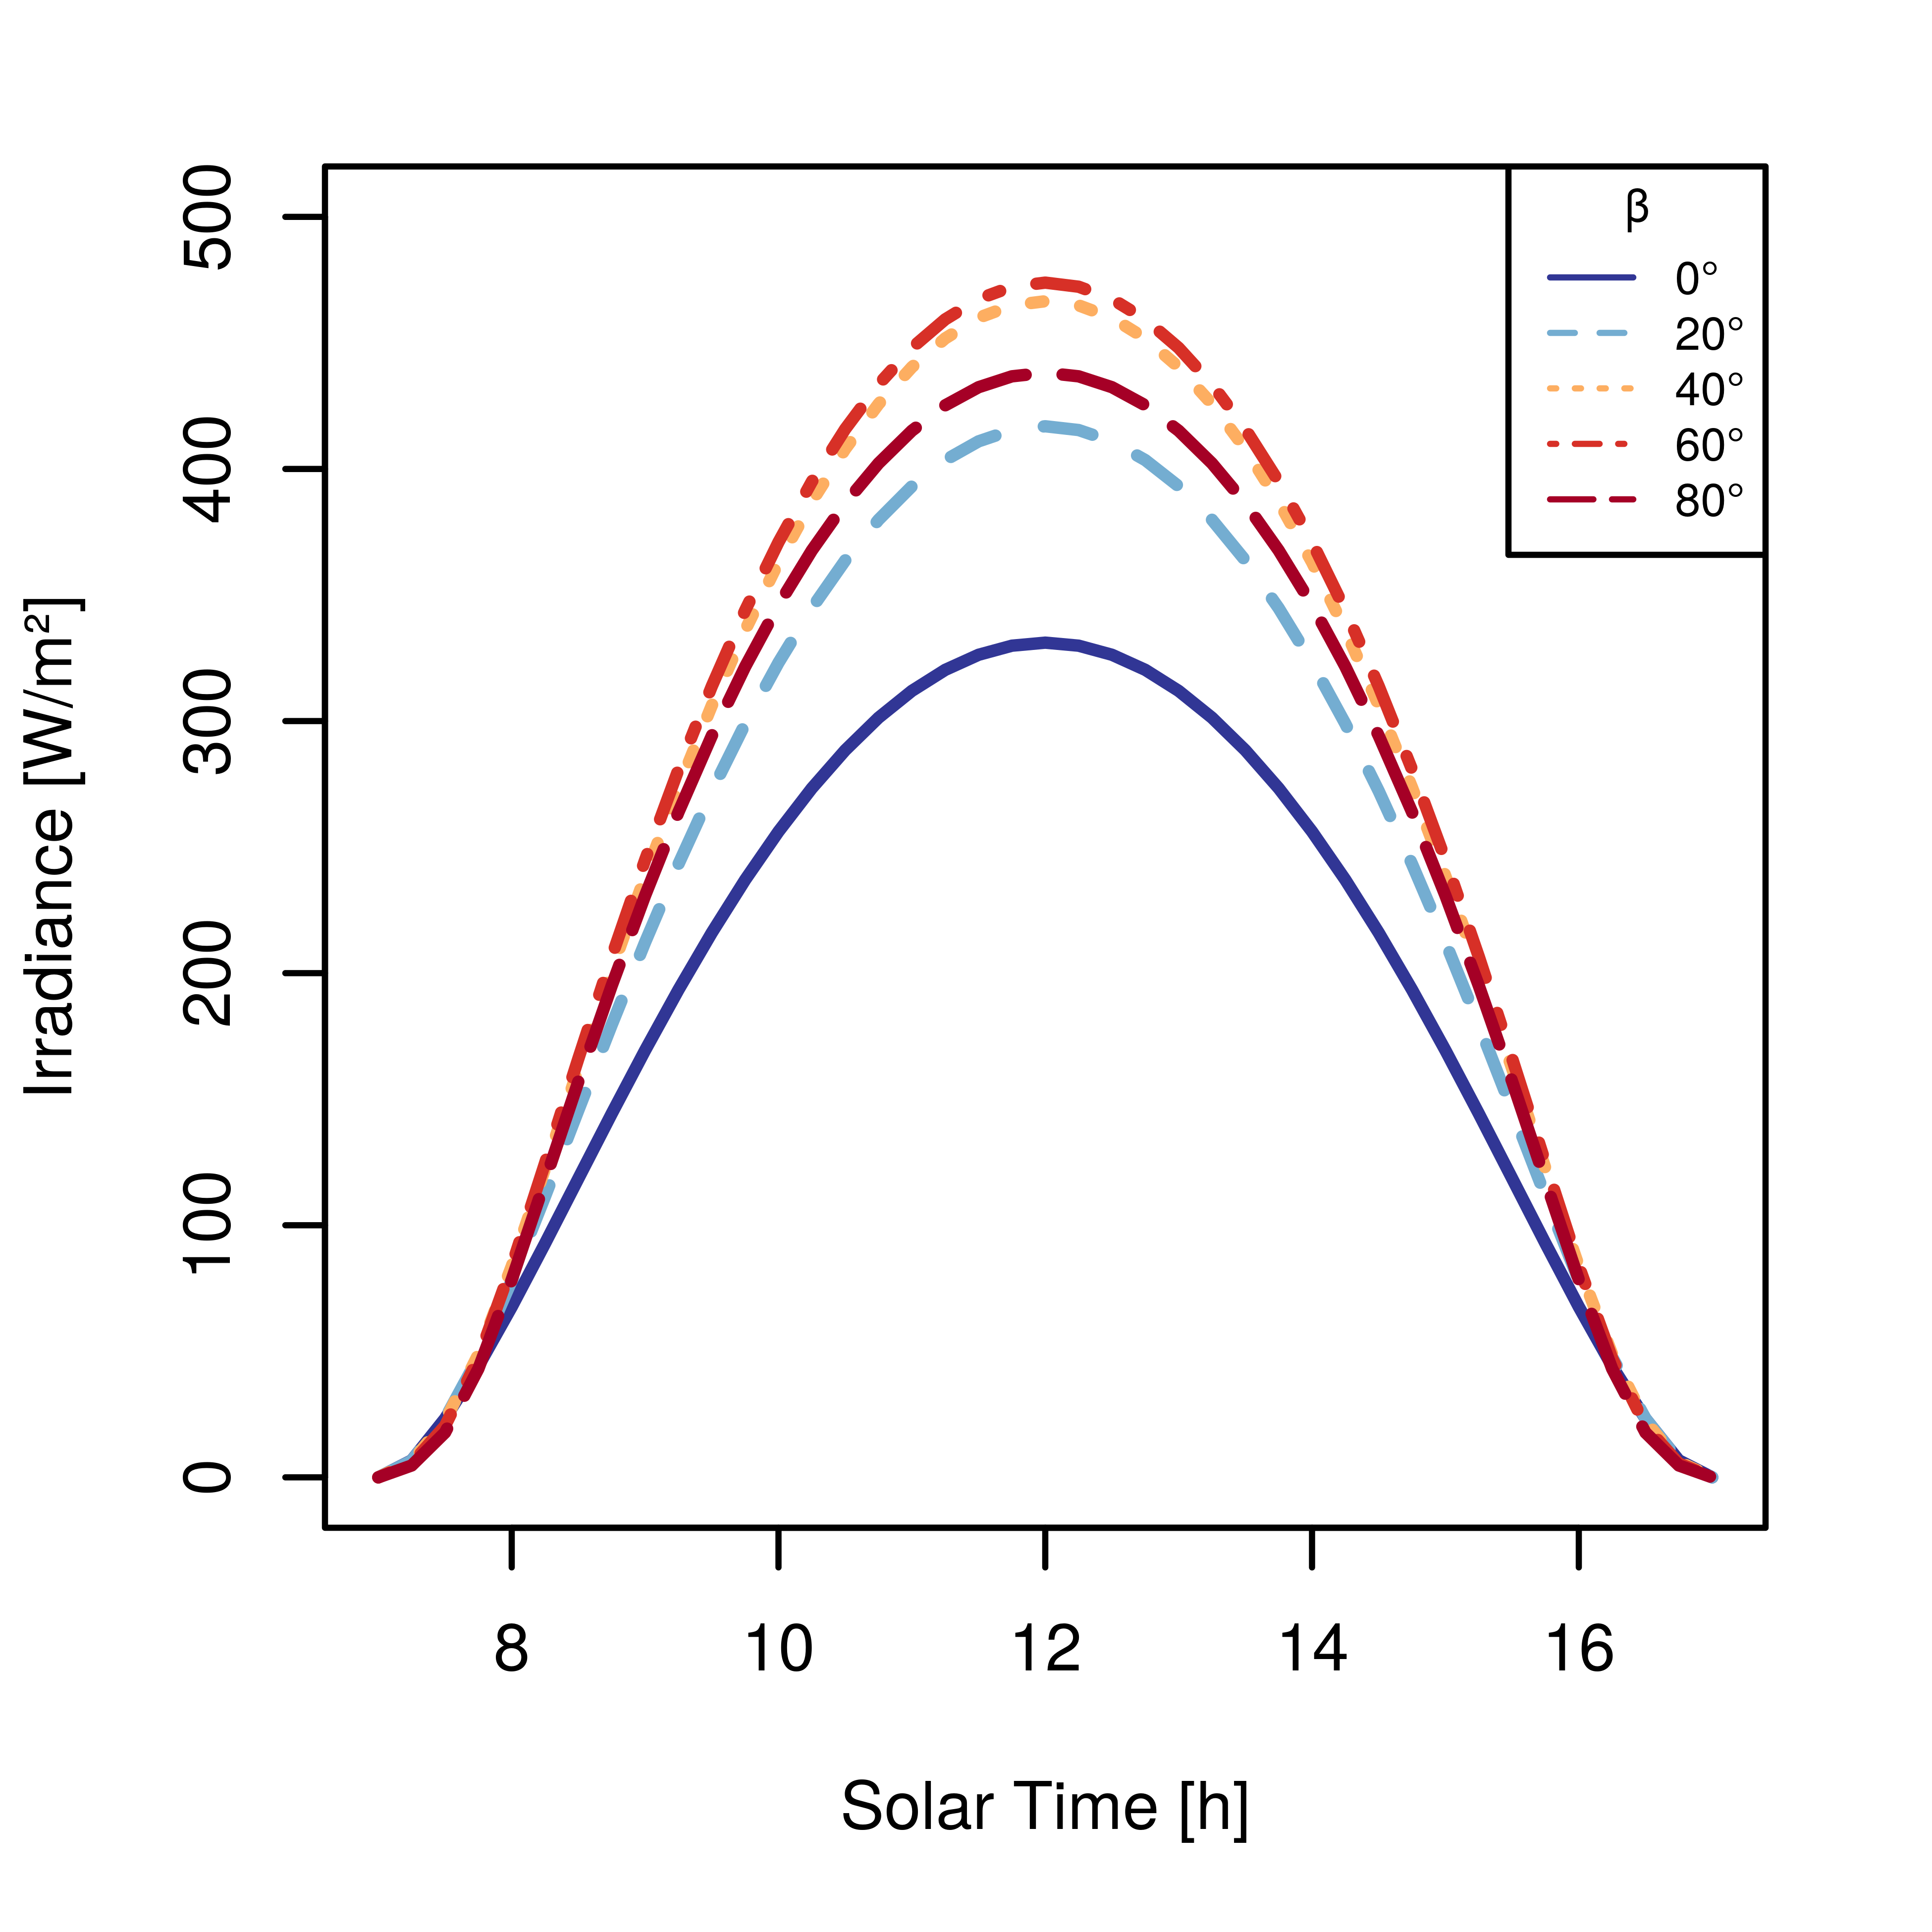
\includegraphics[height=\graphicsHeight]{sections/mars-solar-energy/solar-radiation/plots/gi-variation-for-ls-248-phi-34-tau-04-gammac-south-and-albedo-027.png}
  		\subcaption{$\gamma_{c} = \SI{0}{\degree}$ (South)}
  		\label{fig:sub:irradiance-inclined-gamma-c-0}
  	\end{subfigure}\hfill
    \begin{subfigure}[t]{\subfigureWidth}
      \centering
  		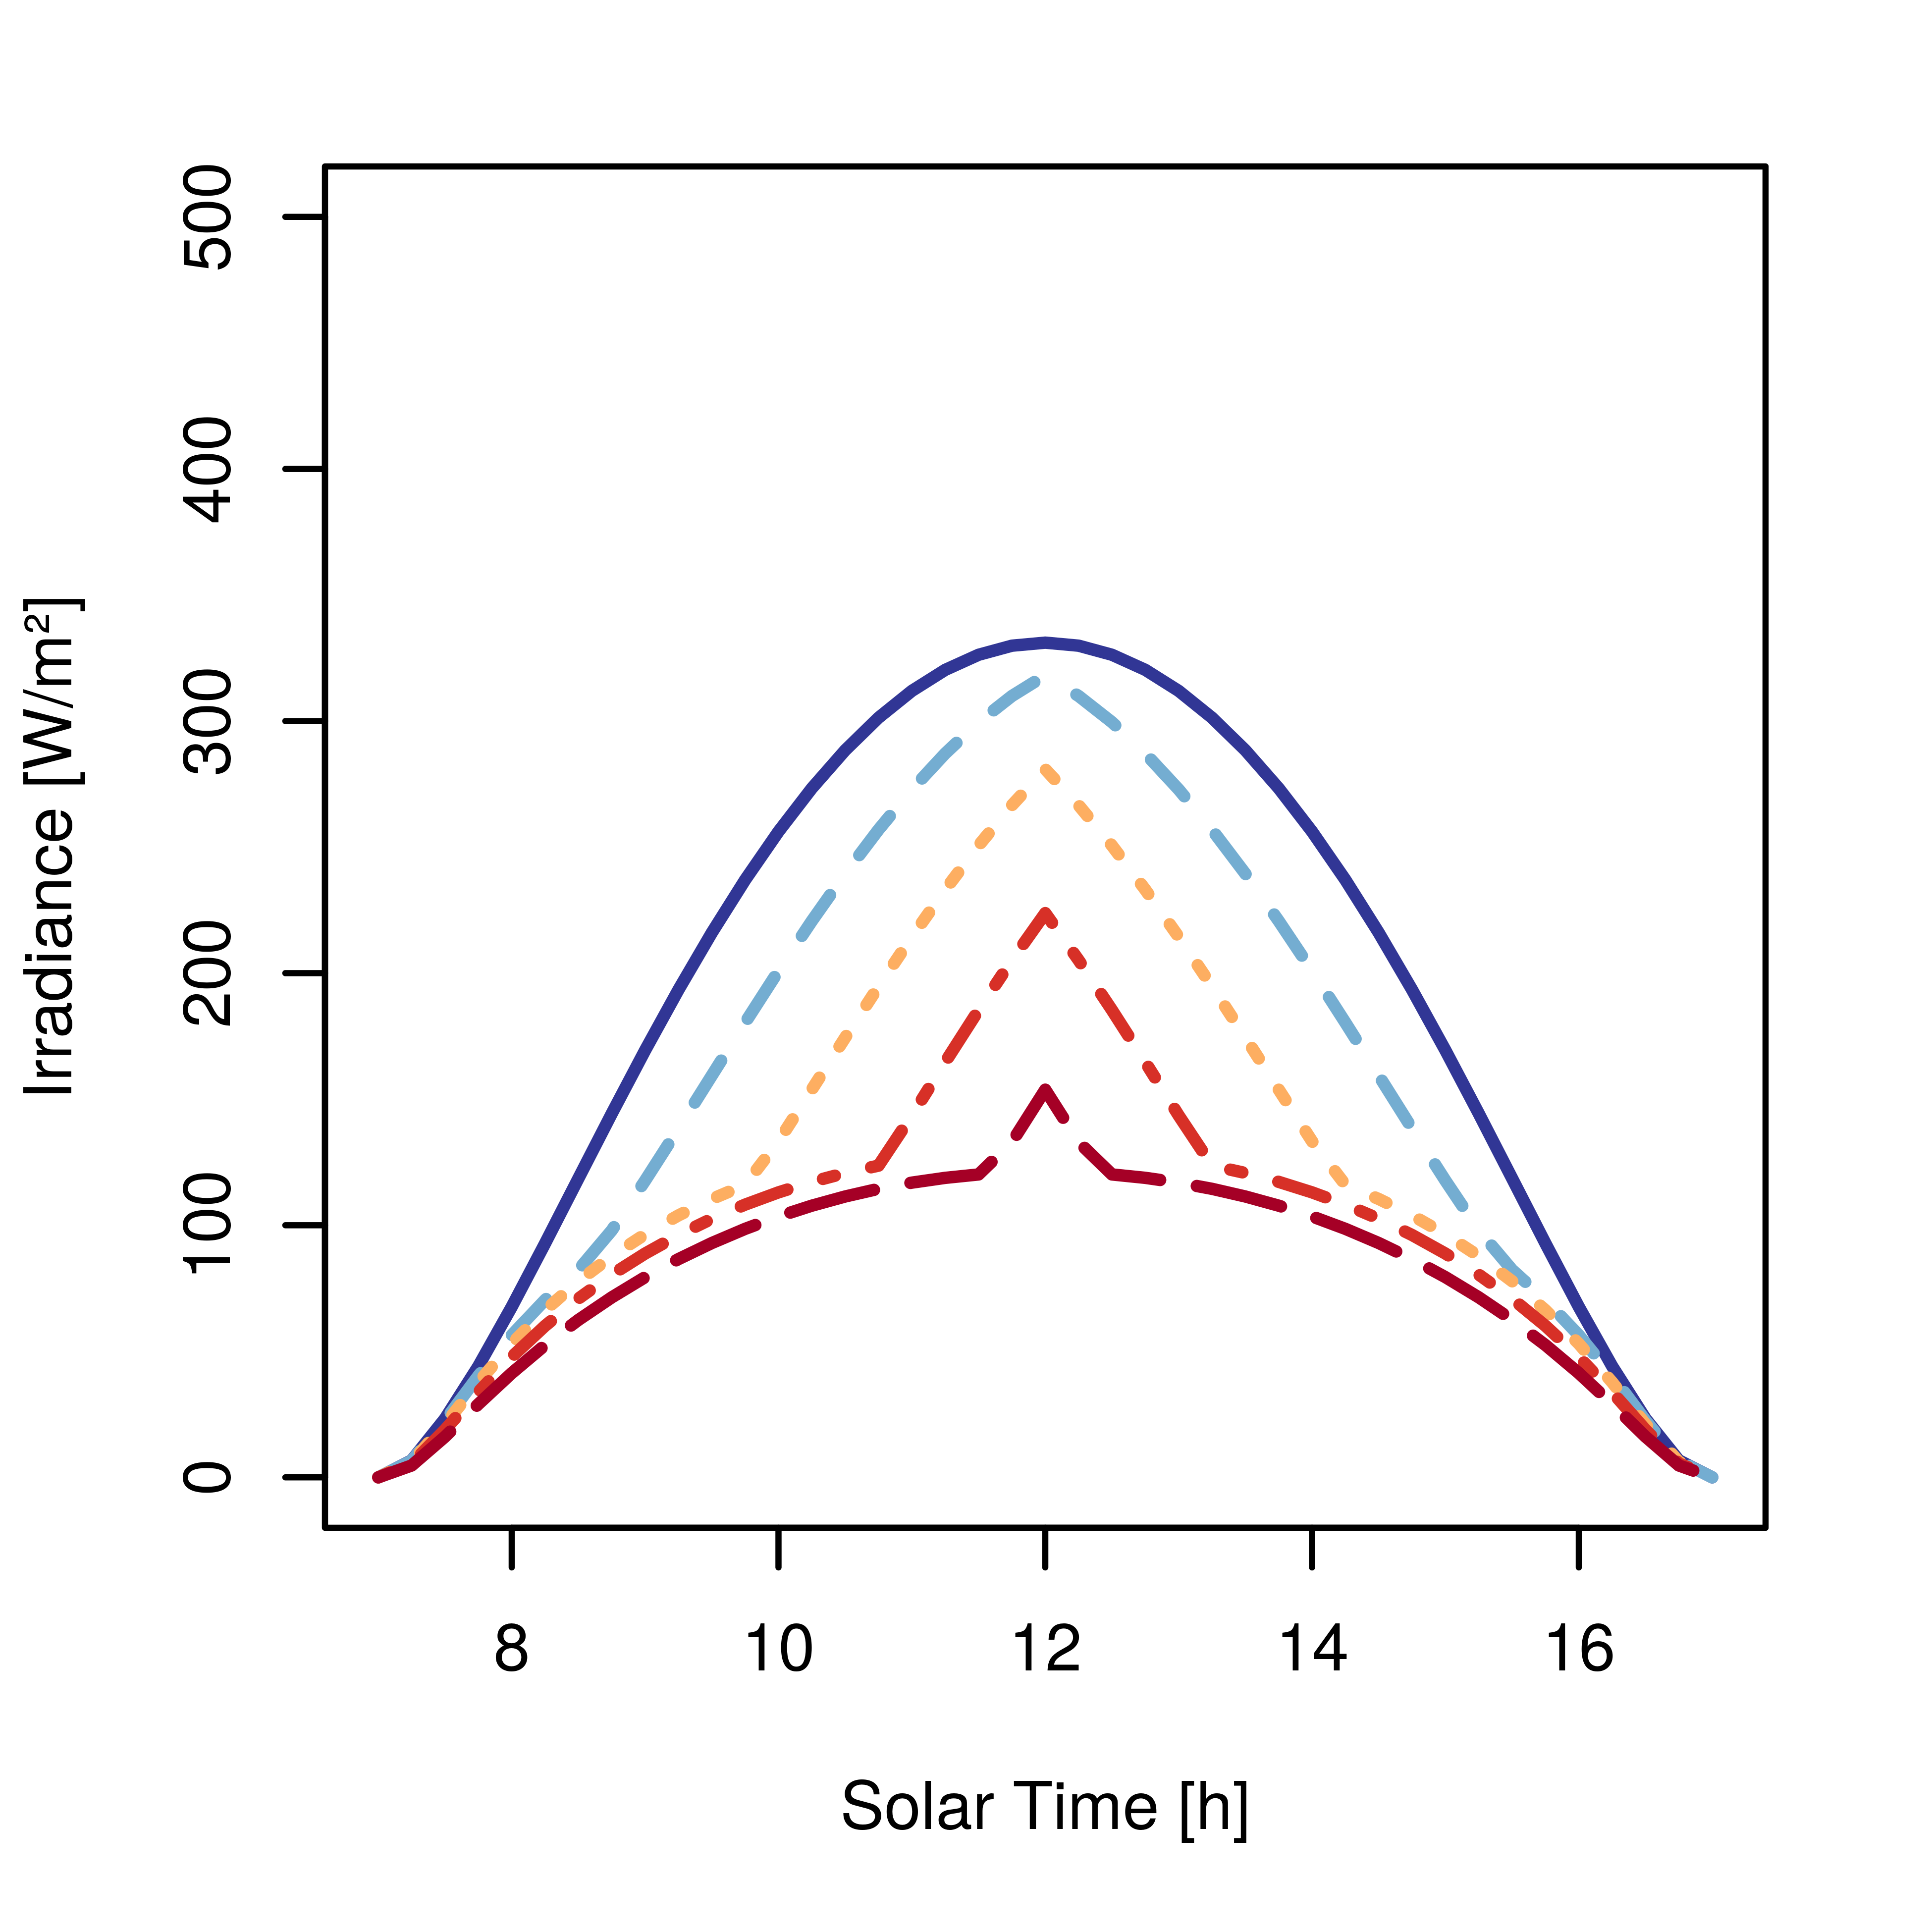
\includegraphics[height=\graphicsHeight]{sections/mars-solar-energy/solar-radiation/plots/gi-variation-for-ls-248-phi-34-tau-04-gammac-east-and-albedo-027.png}
  		\subcaption{$\gamma_{c} = \SI{-90}{\degree}$ (East)}
  		\label{fig:sub:irradiance-inclined-gamma-c-m90}
  	\end{subfigure}\\[0.8ex]
%% 2nd row
    \begin{subfigure}[t]{\subfigureWidth}
      \centering
  		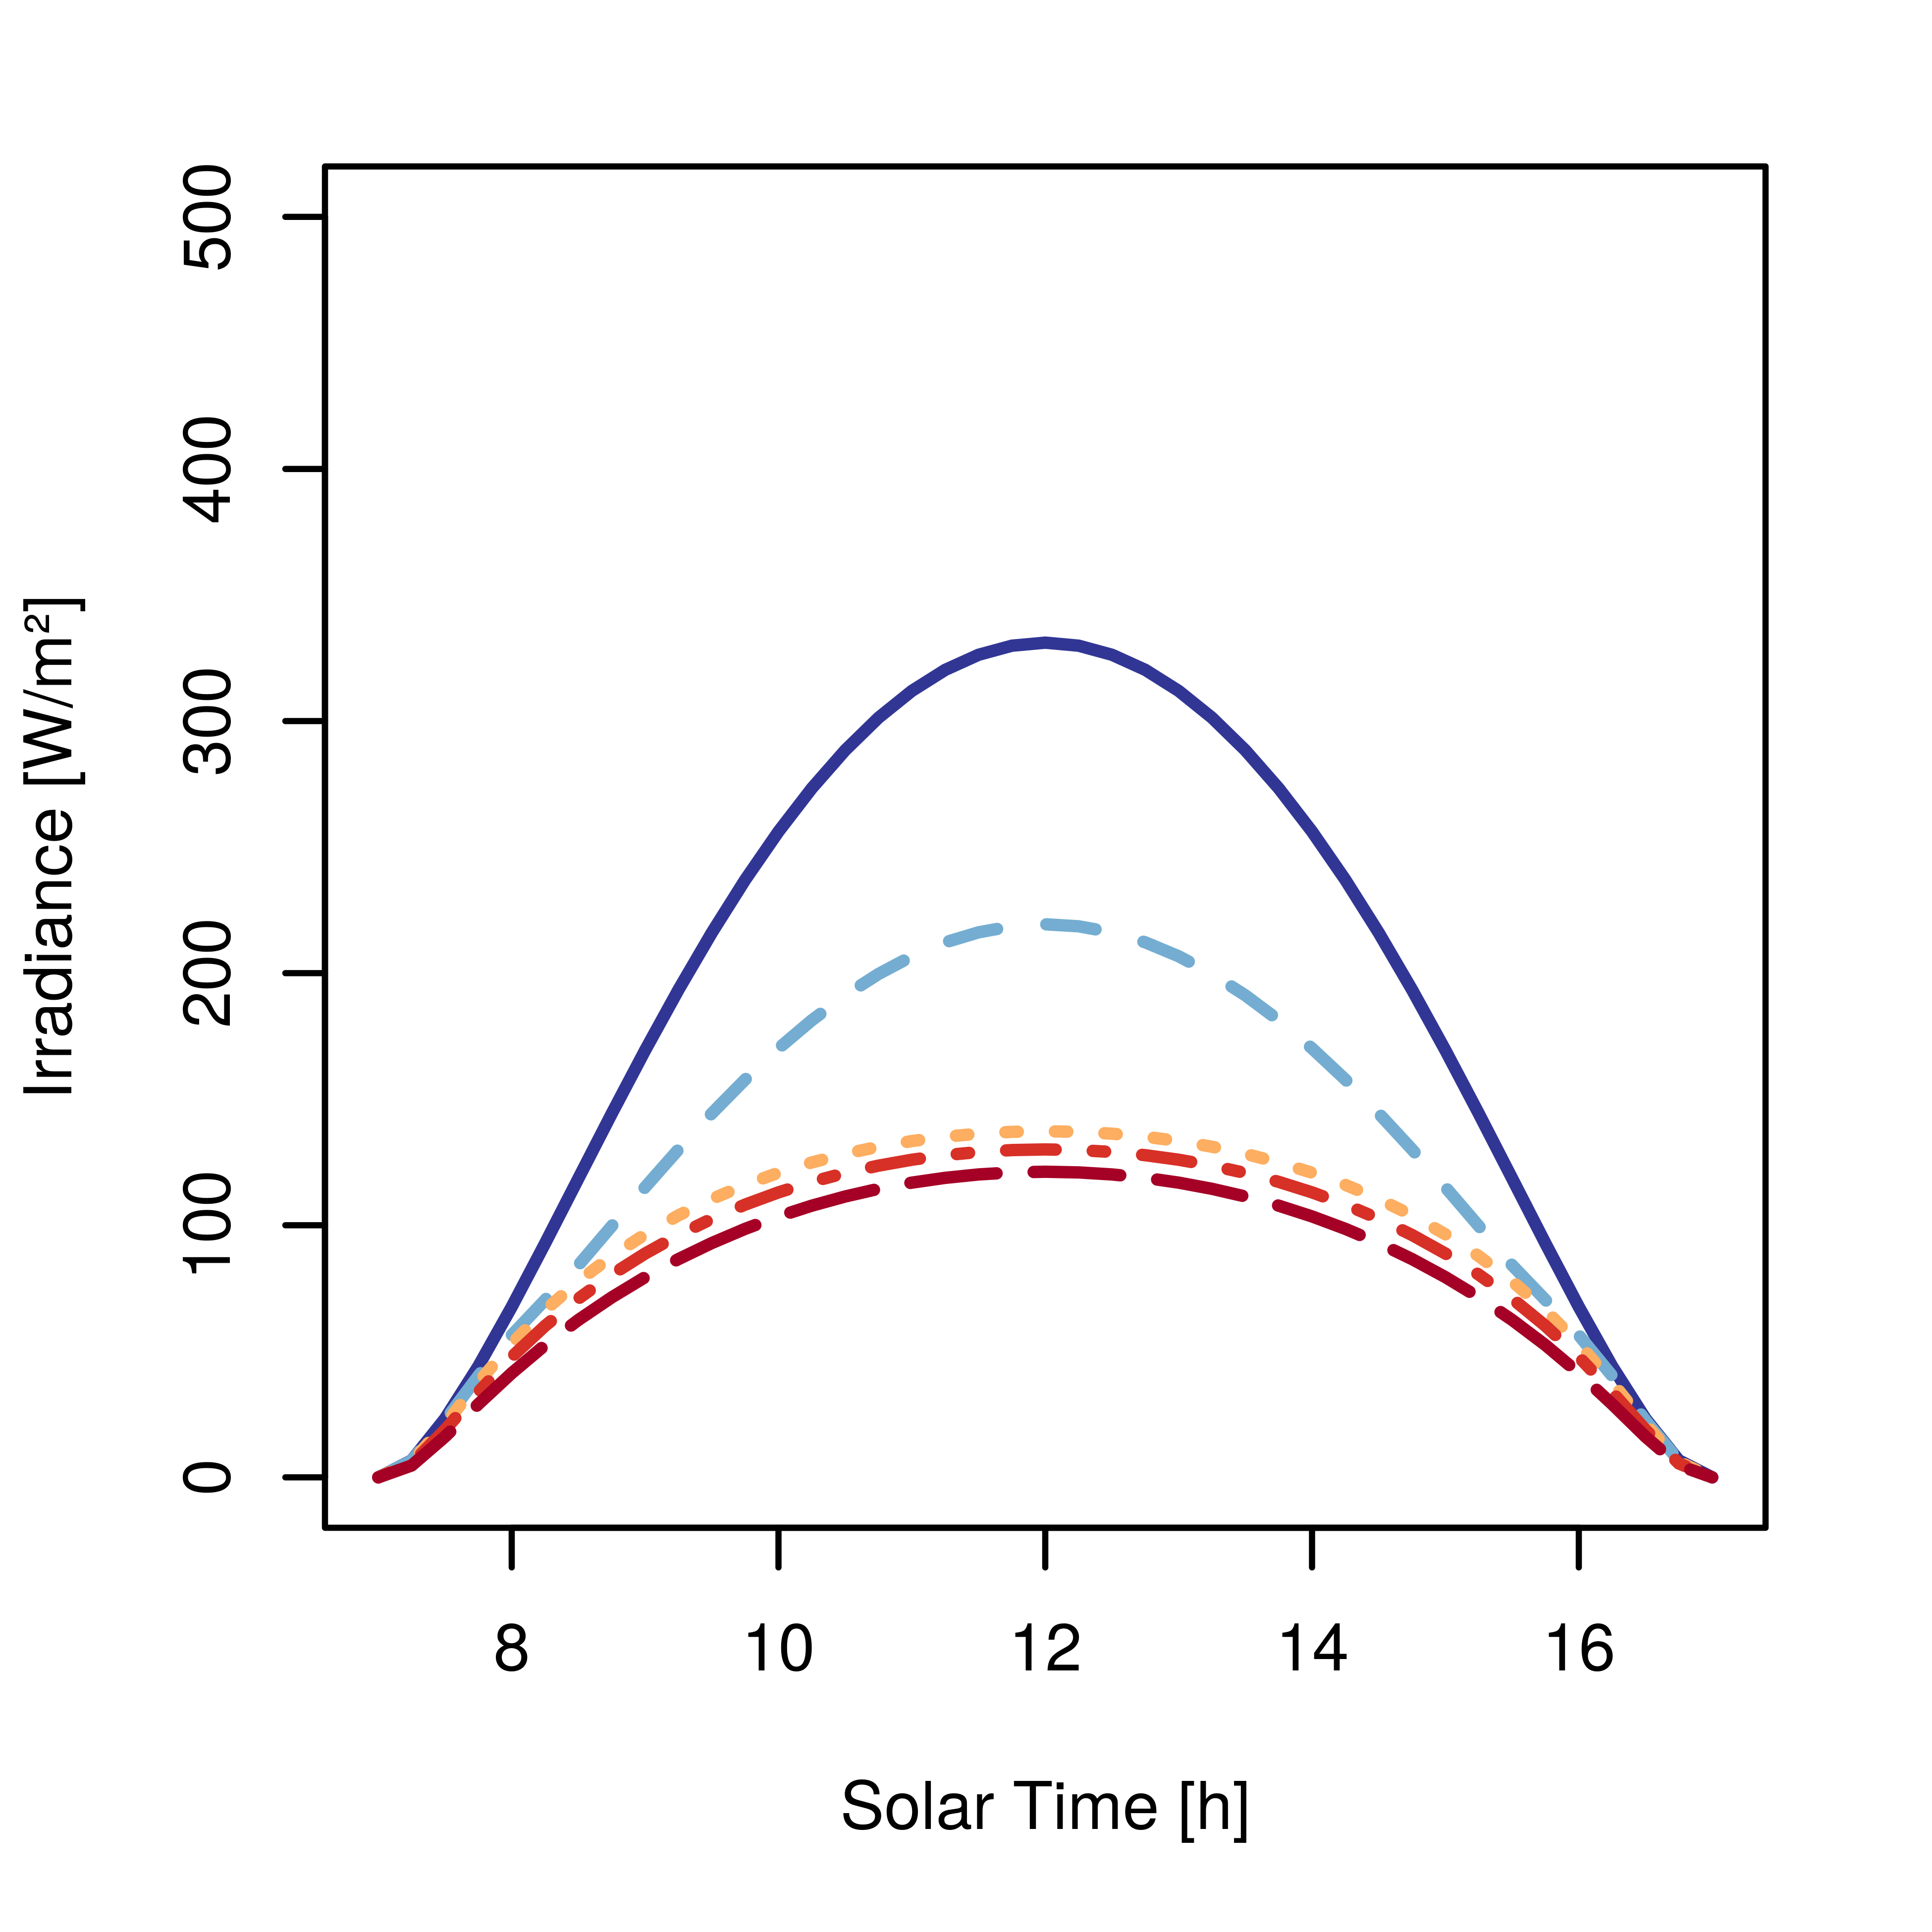
\includegraphics[height=\graphicsHeight]{sections/mars-solar-energy/solar-radiation/plots/gi-variation-for-ls-248-phi-34-tau-04-gammac-north-and-albedo-027.png}
  		\subcaption{$\gamma_{c} = \SI{180}{\degree}$ (North)}
  		\label{fig:sub:irradiance-inclined-gamma-c-180}
  	\end{subfigure}\hfill
	   \begin{subfigure}[t]{\subfigureWidth}
      \centering
  		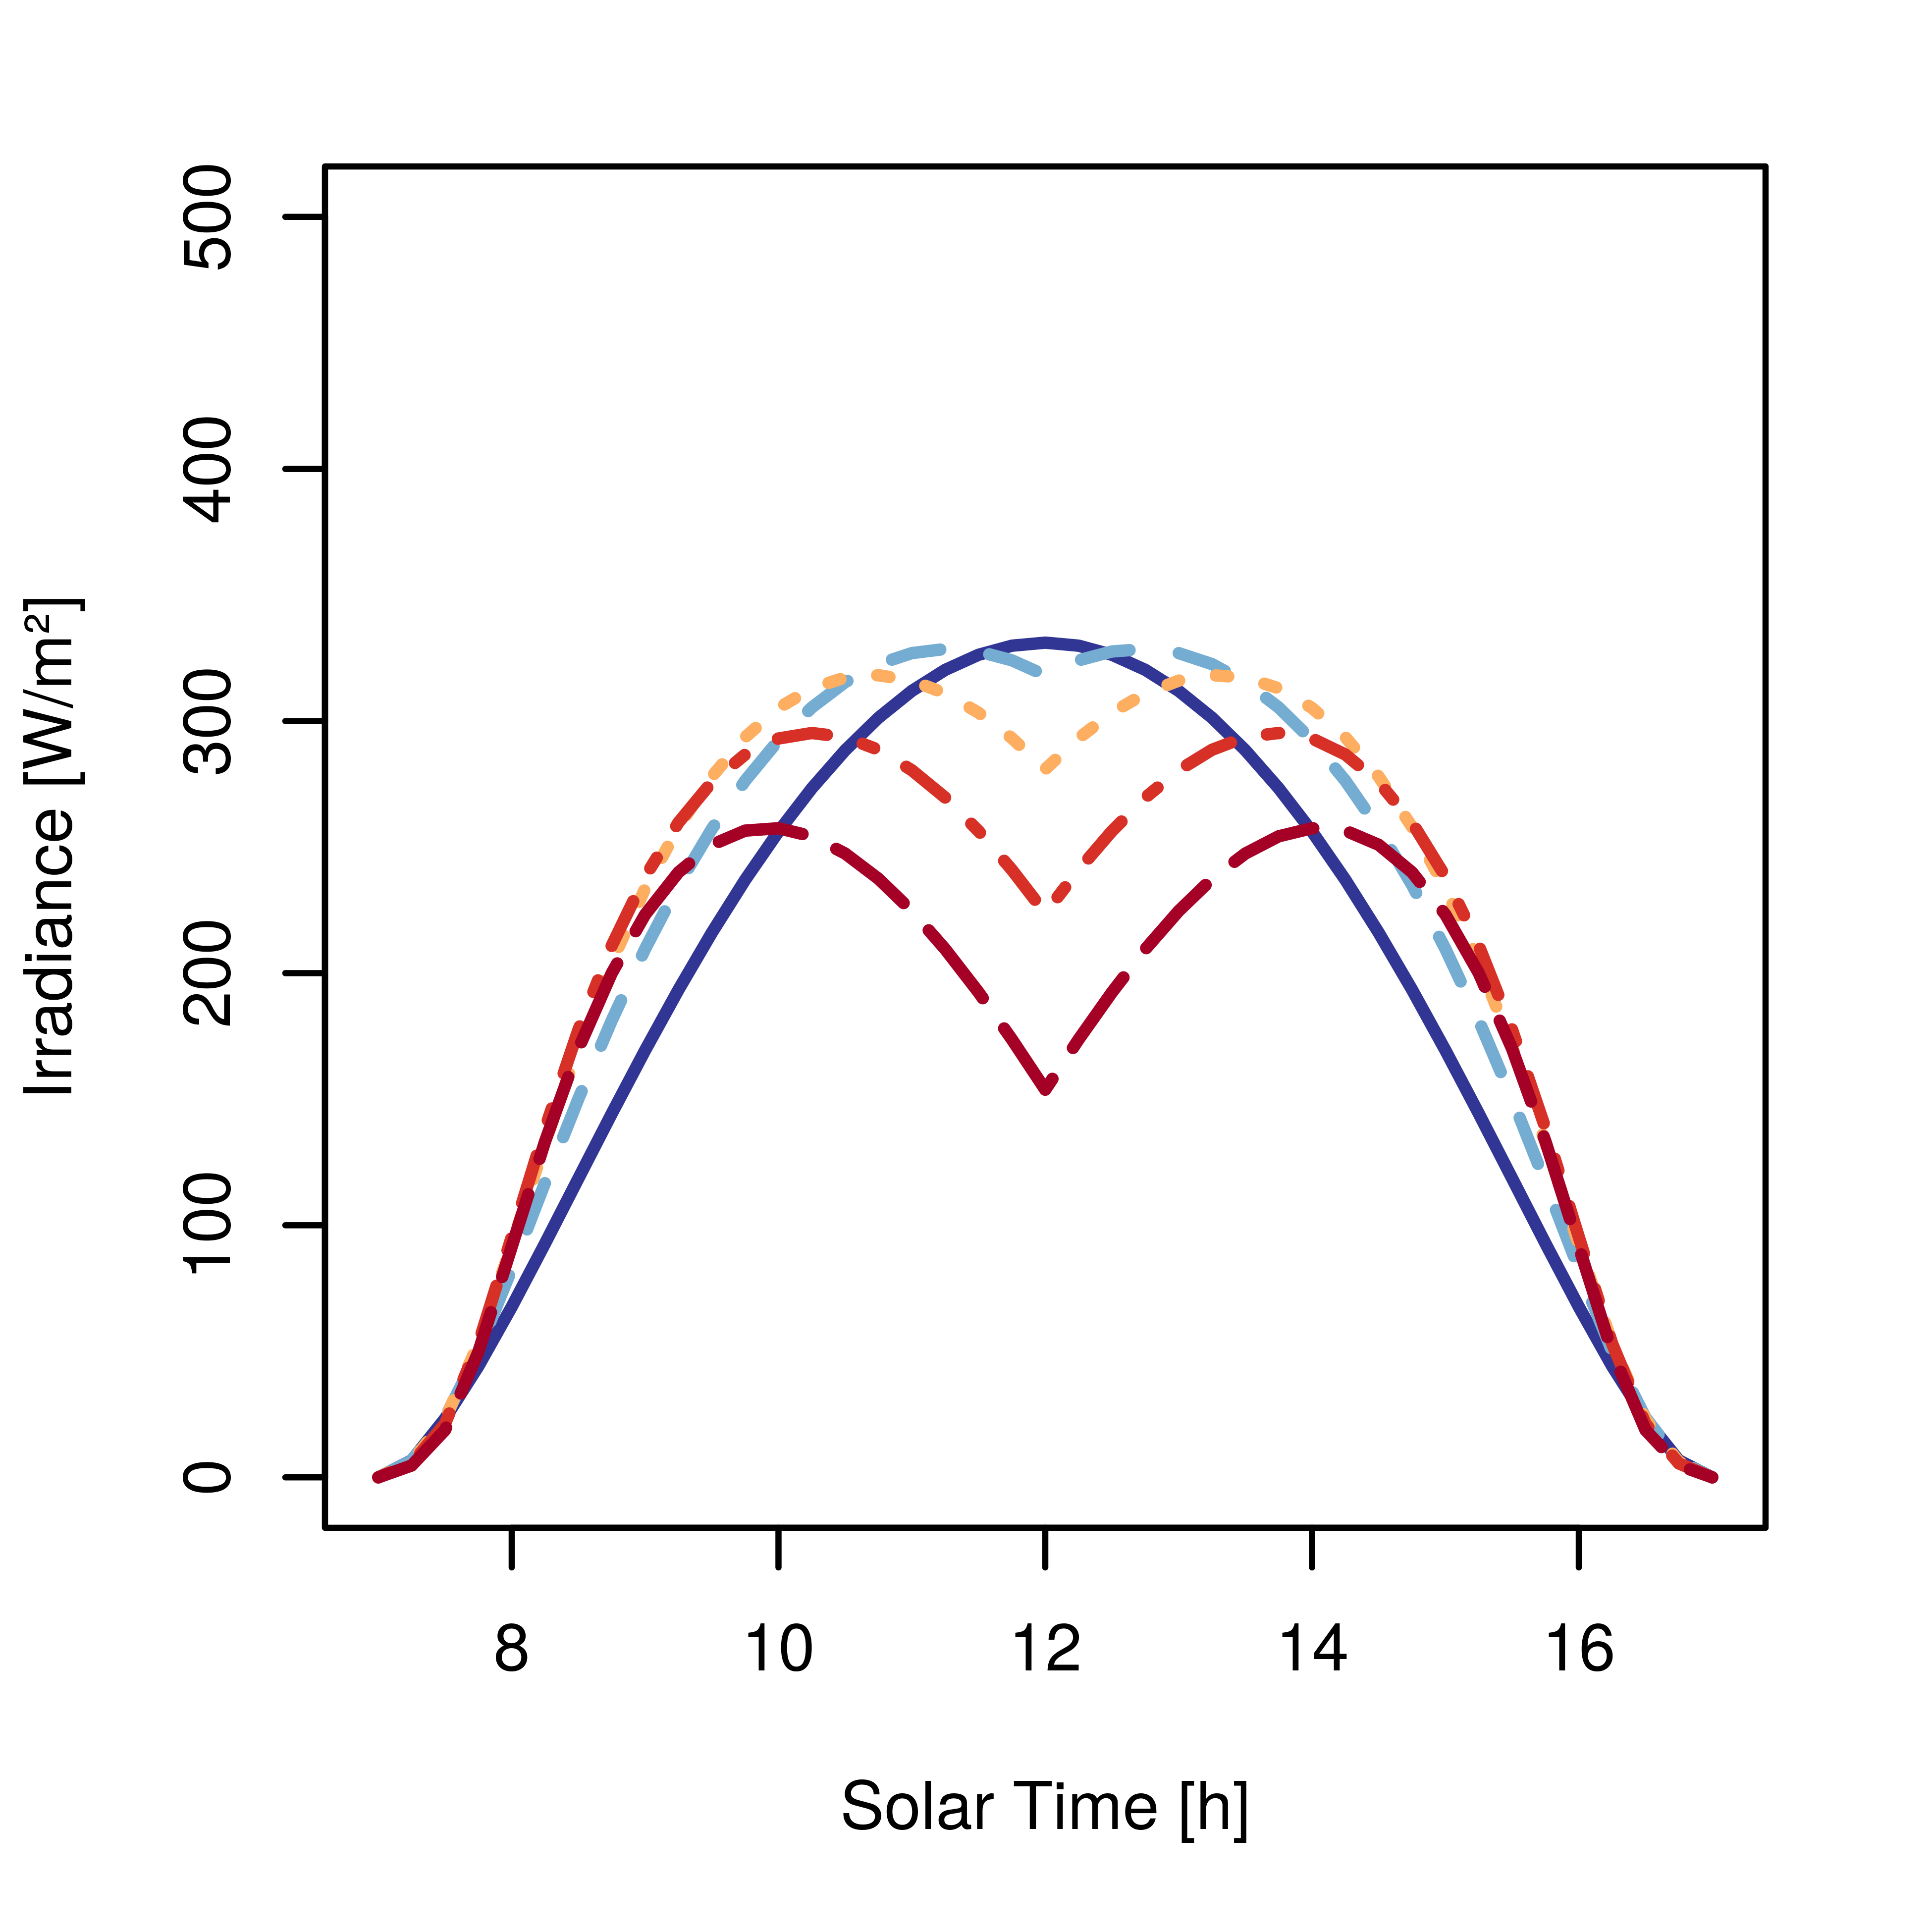
\includegraphics[height=\graphicsHeight]{sections/mars-solar-energy/solar-radiation/plots/gi-variation-for-ls-248-phi-34-tau-04-gammac-west-and-albedo-027.png}
  		\subcaption{$\gamma_{c} = \SI{90}{\degree}$ (West)}
  		\label{fig:sub:irradiance-inclined-gamma-c-90}
	   \end{subfigure}\hfill
	\caption[Global irradiance variations on inclined surface]
    {Diurnal variation of global irradiance on Mars inclined surface for different orientations when $L_{s} = \SI{248}{\degree}$, $\phi = \SI{34}{\degree}$, and $\tau = 0.4$.}
	\label{fig:plot:irradiance-inclined-gamma-c}
\vspace{-2ex}
\end{figure}

\clearpage
Global irradiance variations at the northern hemisphere during the perihelion are shown in \refFig{fig:plot:irradiance-inclined-gamma-c} for different inclination and orientation angles. The influence of the inclination angle is most noticeable when comparing orientations directed southwards, towards the equator, to those oriented northwards, away from the equator.

A surface pointing towards the equator faces the general direction of the Sun. This is observed in \refFig{fig:sub:irradiance-inclined-gamma-c-0} where larger inclinations result in greater irradiances. The steepest inclination does not necessarily result in the greatest irradiance, as seen with $\beta = \SI{80}{\degree}$ compared to $\beta = \SI{40}{\degree}$ and $\beta = \SI{60}{\degree}$. In \refFig{fig:sub:irradiance-inclined-gamma-c-m90}, global irradiances throughout the day are mostly diffuse for highly inclined eastwards oriented surfaces. The beam irradiance only hits the surface around solar noon which results in the noticeable spikes in global irradiance.

The global insolations $I_{\beta}$ on an inclined surface for a given time period and daily global insolation $H_{\beta}$ are obtained by following the same procedure described in \refSec{sec:MartianEnvironment:SolarRadiation:Insolation}. That is to say, obtaining $I_{\beta}$ by integrating \refEqn{eq:G_beta} and integrating $I_{\beta}$ over the period from sunrise to sunset in order to obtain $H_{\beta}$.


\subsection{Summary}
Solar radiation on Mars is made out of beam and diffuse components. Irradiance is mostly diffuse for high $\tau$ factors due to light scattering from airborn dust. A combination of different surface inclination and orientation angles can serve to increase solar irradiance with respect to the position of the Sun. These gains are negligeable when irradiance is mostly diffuse.

%\todo[inline]{TODO: Present plots for diurnal variation of global insolation on Mars inclined surface for different orientations. This is obtained by integrating the global irradiance on Mars incline surface.}

%\todo[inline]{\textbf{TODO:} Emphasize that it doesn't matter which inclination and orientation configuration you have when most of the irradiance is scattered (dusty days).}

%\subsection{Summary}
%\todo[inline]{\textbf{TODO:} Write section summary.}
